%--------|---------|---------|---------|---------|---------|---------|---------|
%       10        20        30        40        50        60        70        80
%-------------------------------------------------------------------------------

\documentclass[11pt, twoside, titlepage, a4paper]{article}
% set utf8 encoding, and set font encoding T1 to allow "|" ">" "<" etc
\usepackage[utf8]{inputenc}
\usepackage[T1]{fontenc}
\usepackage[a4paper,inner=40mm,outer=25mm,top=25mm,bottom=25mm,pdftex]{geometry}
% These page settings give images 1.0\linewidth around 135-140mm wide (ca 138mm)
% meaning a 300dpi image is around 1600 pixels wide
\usepackage{graphicx}   % For eps figures
\usepackage{epsfig}     % Alternative package
\usepackage[hang,small,bf]{caption}

\usepackage[british]{babel}       

\usepackage[yyyymmdd]{datetime}
\renewcommand{\dateseparator}{--}

\usepackage{fancyhdr}
\pagestyle{fancy}
% with this we ensure that the chapter and section
% headings are in lowercase.
%\renewcommand{\chaptermark}[1]{\markboth{#1}{}}  % no "\chapter" in article doc type
\renewcommand{\sectionmark}[1]{\markright{\thesection\ #1}}
\fancyhf{} % delete current setting for header and footer
\fancyhead[LE,RO]{\bfseries\thepage}
\fancyhead[LO]{\bfseries\rightmark}
\fancyhead[RE]{\bfseries\leftmark}
\renewcommand{\headrulewidth}{0.5pt}
\renewcommand{\footrulewidth}{0pt}
\addtolength{\headheight}{0.5pt} % make space for the rule
\fancypagestyle{plain}{%
    \fancyhead{} % get rid of headers on plain pages
    \renewcommand{\headrulewidth}{0pt} % and the line
}


% remove forced implicit vertical whitespace before and after verbatim environment
\makeatletter
\preto{\@verbatim}{\topsep=0pt \partopsep=0pt }
\makeatother


% allow to force indentation of first line in section
% \indent is not working, so workaround \hspace{\parindent} works
\newcommand{\forceindent}{\hspace{\parindent}}


\newcommand{\degrees}{$^\circ$~}
\newcommand{\degree}{$^\circ$}
\newcommand{\ca}{$\approx$}

\newcommand{\vs}{$\backslash\ $}  % "versus" slash
\newcommand{\bs}{$\backslash\ $}  % just backslash


% want clear dash insert commands
\newcommand{\dash}{-}     % just a normal hyphen dash  "-"
\newcommand{\ndash}{--}   % n-dash "--"
\newcommand{\mdash}{---}  % m-dash "---"


%link new command names to the original font sizes,
%for easier to remember smaller font size
\newcommand{\vsmall}{\footnotesize}  % simpler to remember
\newcommand{\vvsmall}{\scriptsize}   %
%\newcommand{\vvvsmall}{\tiny}


\usepackage[colorlinks=true,linkcolor=black,urlcolor=blue]{hyperref}


\usepackage{ifthen}


% \needspace{5\baselineskip}      << reserves approximately 5 lines, leaves raggedbottom, more efficient
% \Needspace{5\baselineskip}      << reserves exactly 5 lines, leaves raggedbottom, less efficient
% \Needpsace*{5\baselineskip}     << leaves flushbottom if \flushbottom is in effect, otherwise ragged
\usepackage{needspace}



% \skill{blabla}
\newboolean{skillsaslist}
\setboolean{skillsaslist}{true}
\ifthenelse{\boolean{skillsaslist}}{\newcommand{\skill}[1]{\item[#1]}}{\newcommand{\skill}[1]{\subsubsection*{#1}}}
\ifthenelse{\boolean{skillsaslist}}{\newcommand{\openskillslist}{\begin{description}}}{\newcommand{\openskillslist}{}}
\ifthenelse{\boolean{skillsaslist}}{\newcommand{\closeskillslist}{\end{description}}}{\newcommand{\closeskillslist}{}}

% \action{blabla}
\newboolean{actionsaslist}
\setboolean{actionsaslist}{true}
\ifthenelse{\boolean{actionsaslist}}{\newcommand{\action}[1]{\item[#1]}}{\newcommand{\action}[1]{\subsubsection*{#1}}}
\ifthenelse{\boolean{actionsaslist}}{\newcommand{\openactionslist}{\begin{description}}}{\newcommand{\openactionslist}{}}
\ifthenelse{\boolean{actionsaslist}}{\newcommand{\closeactionslist}{\end{description}}}{\newcommand{\closeactionslist}{}}

% \eqitem{blabla}
\newboolean{itemsaslist}
\setboolean{itemsaslist}{true}
\ifthenelse{\boolean{itemsaslist}}{\newcommand{\eqitem}[1]{\item[#1]}}{\newcommand{\eqitem}[1]{\subsubsection*{#1}}}
\ifthenelse{\boolean{itemsaslist}}{\newcommand{\openitemslist}{\begin{description}}}{\newcommand{\openactionslist}{}}
\ifthenelse{\boolean{itemsaslist}}{\newcommand{\closeitemslist}{\end{description}}}{\newcommand{\closeactionslist}{}}


\newenvironment{readoutloud}%
{\begin{quote}\begin{itshape}}%
{\end{itshape}\end{quote}}%



% need a nice easily visible TODO marker
\newcommand{\todo}{\textbf{TODO:}~}
\newcommand{\TODO}{\LARGE\textbf{TODO:}\normalsize~}




\begin{document}




%-------------------------------------------------------------------------------
% cover page for work in progress, remove when completed
%-------------------------------------------------------

\pagestyle{empty}
%\vspace{5cm}    -- nope, not honoured at beginning of page ?

\begin{center}
\huge
Goblin Destiny

\vspace{3mm}

\large
Death by GrimGnash

\vspace{4cm}

\normalsize
ongoing campaign\\
work in progress, writing as we go\\

\vfill

\today

\end{center}






%-------------------------------------------------------------------------------
% begin main matter
%------------------
\cleardoublepage
\pagestyle{fancy}

\setcounter{page}{1}


% will mark both left and right pages with an abbreviated section title
% since this is most likely to be read on screens one page at a time instead of
% printed in a binder/book with left/right pages visible simultaneously.
%\markboth{lefttitle}{righttitle}


%\mainmatter  -- nope, not in article




%--------|---------|---------|---------|---------|---------|---------|---------|
%       10        20        30        40        50        60        70        80
%-------------------------------------------------------------------------------
\section*{Goblin Destiny}
\markboth{goblin destiny}{goblin destiny}

A silly campaign, playing Villainous Goblins fighting to survive against long odds.

\

\noindent \textbf{These misadventures} follow the GamGang goblin clan and their struggle to carve out a tiny slice of the world for themselves. Their land and livelihood is invaded by another group of bandits and their Fearless Leader Gamling dies during a highway robbery. The old prophecy of \emph{Death by GrimGnash} is coming true...

\

\tableofcontents                              % sets page header "CONTENT"
\markboth{goblin destiny}{goblin destiny}     % restore the page headers

\vspace{4\baselineskip}

\needspace{15\baselineskip}

\phantomsection\addcontentsline{toc}{section}{introduction}
\subsection*{Introduction}

The campaign should be more fun than serious. Crazy adventures, plans gone wrong, comical stupidity and shortsightedness. Early on the Heroes will improve their situation, gaining loot and experience. As their banditry grows so does the response from the law and order in the region. Patrols are more frequent. Loot is more difficult to sell. Specialised troops start hunting them.
In the end most Heroes will die or flee when they meet GrimGnash. Regardless, the GamGang Clan is no more after GrimGnash is done.

Perhaps even Burmak or Lundqvist manage to root out enough of the gang to close the campaign, but it's more fun if you can balance it on the thin edge so it's difficult, two steps forward, one step back, surival by flight to fight another day.

Goblin life ain't easy!


\subsection*{Campaign outline}

The following adventures make up the main campaign arc. Most are important, but some can be skipped or won't happen depending on the outcome of the previous ones.

\begin{description}

    \item[another day in the office] A short intro fight to get the players oriented with their characters. Just some farmers, guards, and a bit of loot.

    \item[robbery gone wrong] Another band of robbers show up during a routine highway robbery. Gamling dies. GammelTant is the new Leader and calls for Revenge! She recognises the first sign of the Dread Prophecy of \emph{Death by GrimGnash}.

    \item[kill the bandits] The murderous invaders must be killed. Their camp has been scouted. An attack in the middle of the night is the brilliant idea to revenge Gamling and kill off the competition.

    \item[defend hoom-hool] The Horrible Hoomans have banded together and hired some adventurers to root out the goblin clan. The Heroes must defend their Hoom Hool cave.

    \item[flee and relocate] The Horrible Hoomans try again and again, eventually they succeed. Forcing the goblins to flee and find somewhere else to nest.

    \item[clean the new home] Every new home needs a proper clean up. Get rid of all those pesky spiders, worms, balrogs, and other monsters living there.

    \item[grimgnash] They go to certain death when they to kill GrimGnash to escape the \emph{Death by GrimGnash} prophecy. Perhaps a few characters flee and survive for future adventures, perhaps they all die.

\end{description}


Below are small intermission adventures that are not part of the main campaign and can usually be played at any time. Insert where suitable.

\begin{description}

    \item[patrols] When travelling the gang runs into patrols. Discuss, bluff, bribe, or fight. The patrolmen are not automatically confrontational. If the gang can pass for traders, travellers, or other civilians they can even get some information, or an escort on their way.

    \item[iffygriff eggs] They have spotted iffygriffs flying to an area in The Moors. An old outpost has an iffygriff nest, a small bandit gang, and a haunted guard tower with a cursed sword.

    \item[mutamonsters] A magical place in the forest which turns goblins and critters into strange monsters. They can fight their way to the magic source and get strange mutated abilities and magic-ified equipment.

    \item[torture dungeon] They have found a treasure map pointing to somewhere in the Duns. Ruins of a tower with an old torture dungeon below filled with undead, black bugs, a strange trap, and some loot.
    
    \item[mountain hools] The central mountains hold a few caves. Occupied of course, but perhaps suitable for the relocating clan after agressive negotiations.

    \item[plunder] Perhaps a few road side ambushes or village periphery raids to gather some wealth?

    \item[fishy burglary] They have heard that a Richy Rich is staying in the tavern \emph{Sleeping with the Fishes}. Must be worth sneaking in and plunder his room and stuff.

    \item[shopping] At some point they might want to go shopping for food or gear, or to sell some loot. Who knows what can be found in a nearby village? Some soldiers perhaps?

\end{description}

The Heroes can also go on other adventures, extra raids, weekend shopping sprees, etc. As long as they have enough food to feed GamGang they are more or less free to do what they want. But when GammelTant's stomach starts growling it's dangerous to be around the cook pot empty handed ...


\subsection*{The GamGang clan}

Gamling leads the Gang with an iron fist and empty head. GammelTant is smarter but will not be leading until after Gamling dies.
At the start of the campaign the GamGang crowd is made up of approximately 20 goblins, including Heroes, and some 10+ runts, wolves, critters, etc. 

The whole gang, including heroes, require lots of food each day. Food scarcity, lack of money, lack of good loot, etc, should be common and urgent for most, if not all, of the campaign. Gamling and GammelTant will get angry when the food runs low, and in the end start cooking the goblins or runts they dislike the most, including obnoxious Heroes.

Generally the life in the bandit gang is simple. You help find food and loot. Steal, hunt, gather, or whatnot. You avoid ending up in the cook pot. And you do this until dead.


\subsection*{Goblin Destiny\,\textendash\,\emph{Death by GrimGnash}}
% \, is a small non-breakable, non-disappearing space
% \textendash is an en-dash, smaller than em-dash

The prophecy says that when The Great Leader dies by The Blue Boss, the GamGang must kill GrimGnash or be themselves destroyed.

GrimGnash is a dragon and there is no way in hell the Goblins will win that fight. Thus, the destiny of the goblins is to die! \emph{Mostly}. Some might escape and appear in later campaigns.


\subsection*{What's with Goblins?}

Playing a goblin band is a bit different from a regular group of adventurers. Goblins are lazy, cowardly, blood thirsty, often hungry, live day to day and are poor planners.

Finding enough food should be an issue. This pushes the Heroes to never sit still for long. They will often be tasked with feeding the whole gang, and even though Gamling has money in the coffer he won't give any to the Heroes to buy food.

Try to have smart enemies flee when things turn sour. Less loot, money, and food. A slain human is a delicacy and can feed the whole gang for a day.

Remember that goblins don't speak Common by default. Don't remind them. If none of the Heroes bothered to learn Common they won't be able to communicate with most humans. And if they have low Common skill let them roll for the communication and be merciless with injecting misunderstandings and misinterpretations. Hilarious. 
% see mail 180115

Some goblins even have very low Svartlingo skills. They can't understand or communicate complex sentences or unusual topics easily. Have the players use only simple words, pigin grammar, short sentences, and so on.

\begin{quote}
\begin{small}

On their way to Sleepy Cove, two wagons with eight brave goblins roll north over the grassland. Barely an hour after they've crawled out of their potato sack sleeping bags, eaten some cold snails, and gotten under way. In the distance they see a small group of humans approach. A man on horse and three more walking, relaxed. Closing slowly they carry spears and shields, uniformed. The man on horse rides ahead a little bit and and waves to the goblins as he approaches from a distance.

\begin{description}

\item[Fizzleflare:] \vsmall (svartlingo) \small
"He waves his reinforcements, have to kill'im qick!"

\item[Patrolman rider:] \vsmall (common, shouts from distance) \small 
"Hi. Hi. Hello over there!"

\item[GamGang:] \vsmall (svartlingo, giggling amongst themselves) \small 
"Slaughter smashing! Hehe!"

\item[Heidiblast:]
"I'll prepare a black bolt! Will blow his head clean off!"

\end{description}
... the patrol squad approaches casually ...
\begin{description}

\item[Patrolman rider:] \vsmall (common) \small
"Hi there Happy Tradesmen, how's the beautiful morning treating you? What lovely sunshine we have! And to think that Sanna the Seer claimed it would rain. Haha."

\item[Old Maz:] \vsmall (fail common, broken svartlingo) \small
"What 'im say?"

\item[Kizraz:] \vsmall (fail common, broken svartlingo) \small
"Clue no have. No-Know."

\item[Grapplebottom:] \vsmall (fail common, broken svartlingo) \small
"What understand? Speak Talk?"

\end{description}
... and so on until Fizzleflare manages to understand ...
\begin{description}

\item[Fizzleflare:] \vsmall (broken common) \small
"We come southfrom. Fishesh. Go Sleepy Cove."

\item[Patrolman rider:] \vsmall (common) \small
"Ah. How nice! Please be careful when travelling the area south of town. There is a band of horrible goblin bandits in the woods. Hjalmar Hjälte is in Sleepy Cove gathering a posse to go deal with them. He think they live out of the old goblin warren which Datarian, Maras, and Nostromo cleaned out before the Big Demon Rampage. But why are you coming this strange way?"

\item[Old Maz:] \vsmall (fail common, broken svartlingo) \small
"What say he?"

\item[Kizraz:] \vsmall (fail common, broken svartlingo) \small
"No understand gabbadigook!"

\item[Fizzleflare:] \vsmall (broken common) \small
"Öööh-hum. Big Bandit! Attacked! SturSkurk! Blue Sword. Orcsesh and Fishesh."

\item[Patrolman rider:] \vsmall (common) \small
"Another bandit? Oh no! We don't have enough patrols out on the roads these days. Not since Baron Conq and Pawa clashed after the Demon Rampage. SturSkurk? With Blue Swords and fishing orcs? Apologies, I don't quite understand?"

\end{description}
Meanwhile, the Röbank brothers walk up to the rider and looks at his horse.
\begin{description}

\item[Dunkab Röbank:] \vsmall (fail common: "Hey! Give us horse or we beat the blood out of you:") \small
== "Hurru! Hours-yet grave ooze! Moor ley banshee blood lay Flanders!"

\item[Patrolman rider:] \vsmall (common) \small
"Uhm? Excuse me. I didn't quite understand. Could you please repeat that?"

\end{description}

And here Smashesh Röbank has lost his patience and bashes the horse in the head with his large club. So the murdering begins!

After a surprisingly quick fight the goblins have a wounded horse and four human cadavers to feast on. They promptly forget to continue to Sleepy Cove to trade and instead turn back to Hoom Hool to celebrate.

\end{small}
\end{quote}






\subsection*{Practicalities}

Goblins are squishy but numerous. Each player controls two goblins simultaneous. This is fun and different but an impractical design on my part. Play testing with up to six players controlling two Heroes each, plus sidekicks, meant very large and thus slow fights for part of the campaign. To keep the speed up consider using simplified rules or have the players control only one goblin each and scale the opposition accordingly. \emph{But,} some of the fights are spectacular when the players have a small army of crazy goblins to throw around. The main playthrough was done with 8-20 Heroes and sidekicks on the board at all times.

As the Heroes die off roll replacement goblins with (85+1D10)\% of the the xp of the dead one. The first two goblins should come from a set of five, then each new one from a new set of three.

For players that absolutely don't want to play goblins, have them play a single Hero from another race. Choose a race and roll a small set of characters from that race only (human 2, dwarf 2, elf 1, halfling 2, orc 2). Any elf here should probably have a mental disability to live in a goblin gang, or perhaps they are anthropologists studying the life of the native lesser races?

It can be fun to allow all the goblins to have the effect of infinite prescient training. I.e: they can spend xp to learn skills at any time, not just in between sessions or adventures. This makes for a lot of comedy situations. E.g: \emph{Oh Sh*t! I'm about to die! I'll buy possum to 8.}


\subsection*{This corner of the world}

GamGang is new to the region. They have fled from unknown southlands after being chased out by orcs. On their way north they found two battered goblins. The two used to belong to a bandit gang who had a great hool in the bountiful forest south of Sleepy Cove. Then some Hooman Heroes came and slauhtered most of them a while back. After Gamling promises them a place in GamGang they tell him all about their Bestest LootSpot, Hoom Hool, Skaary plains, Hoomans, etc. GammelTant then promptly wrings their necks and cooks them. The gang was short on food, as usual, and goblins are decent eating.

\begin{figure}[h!]
  \centering
  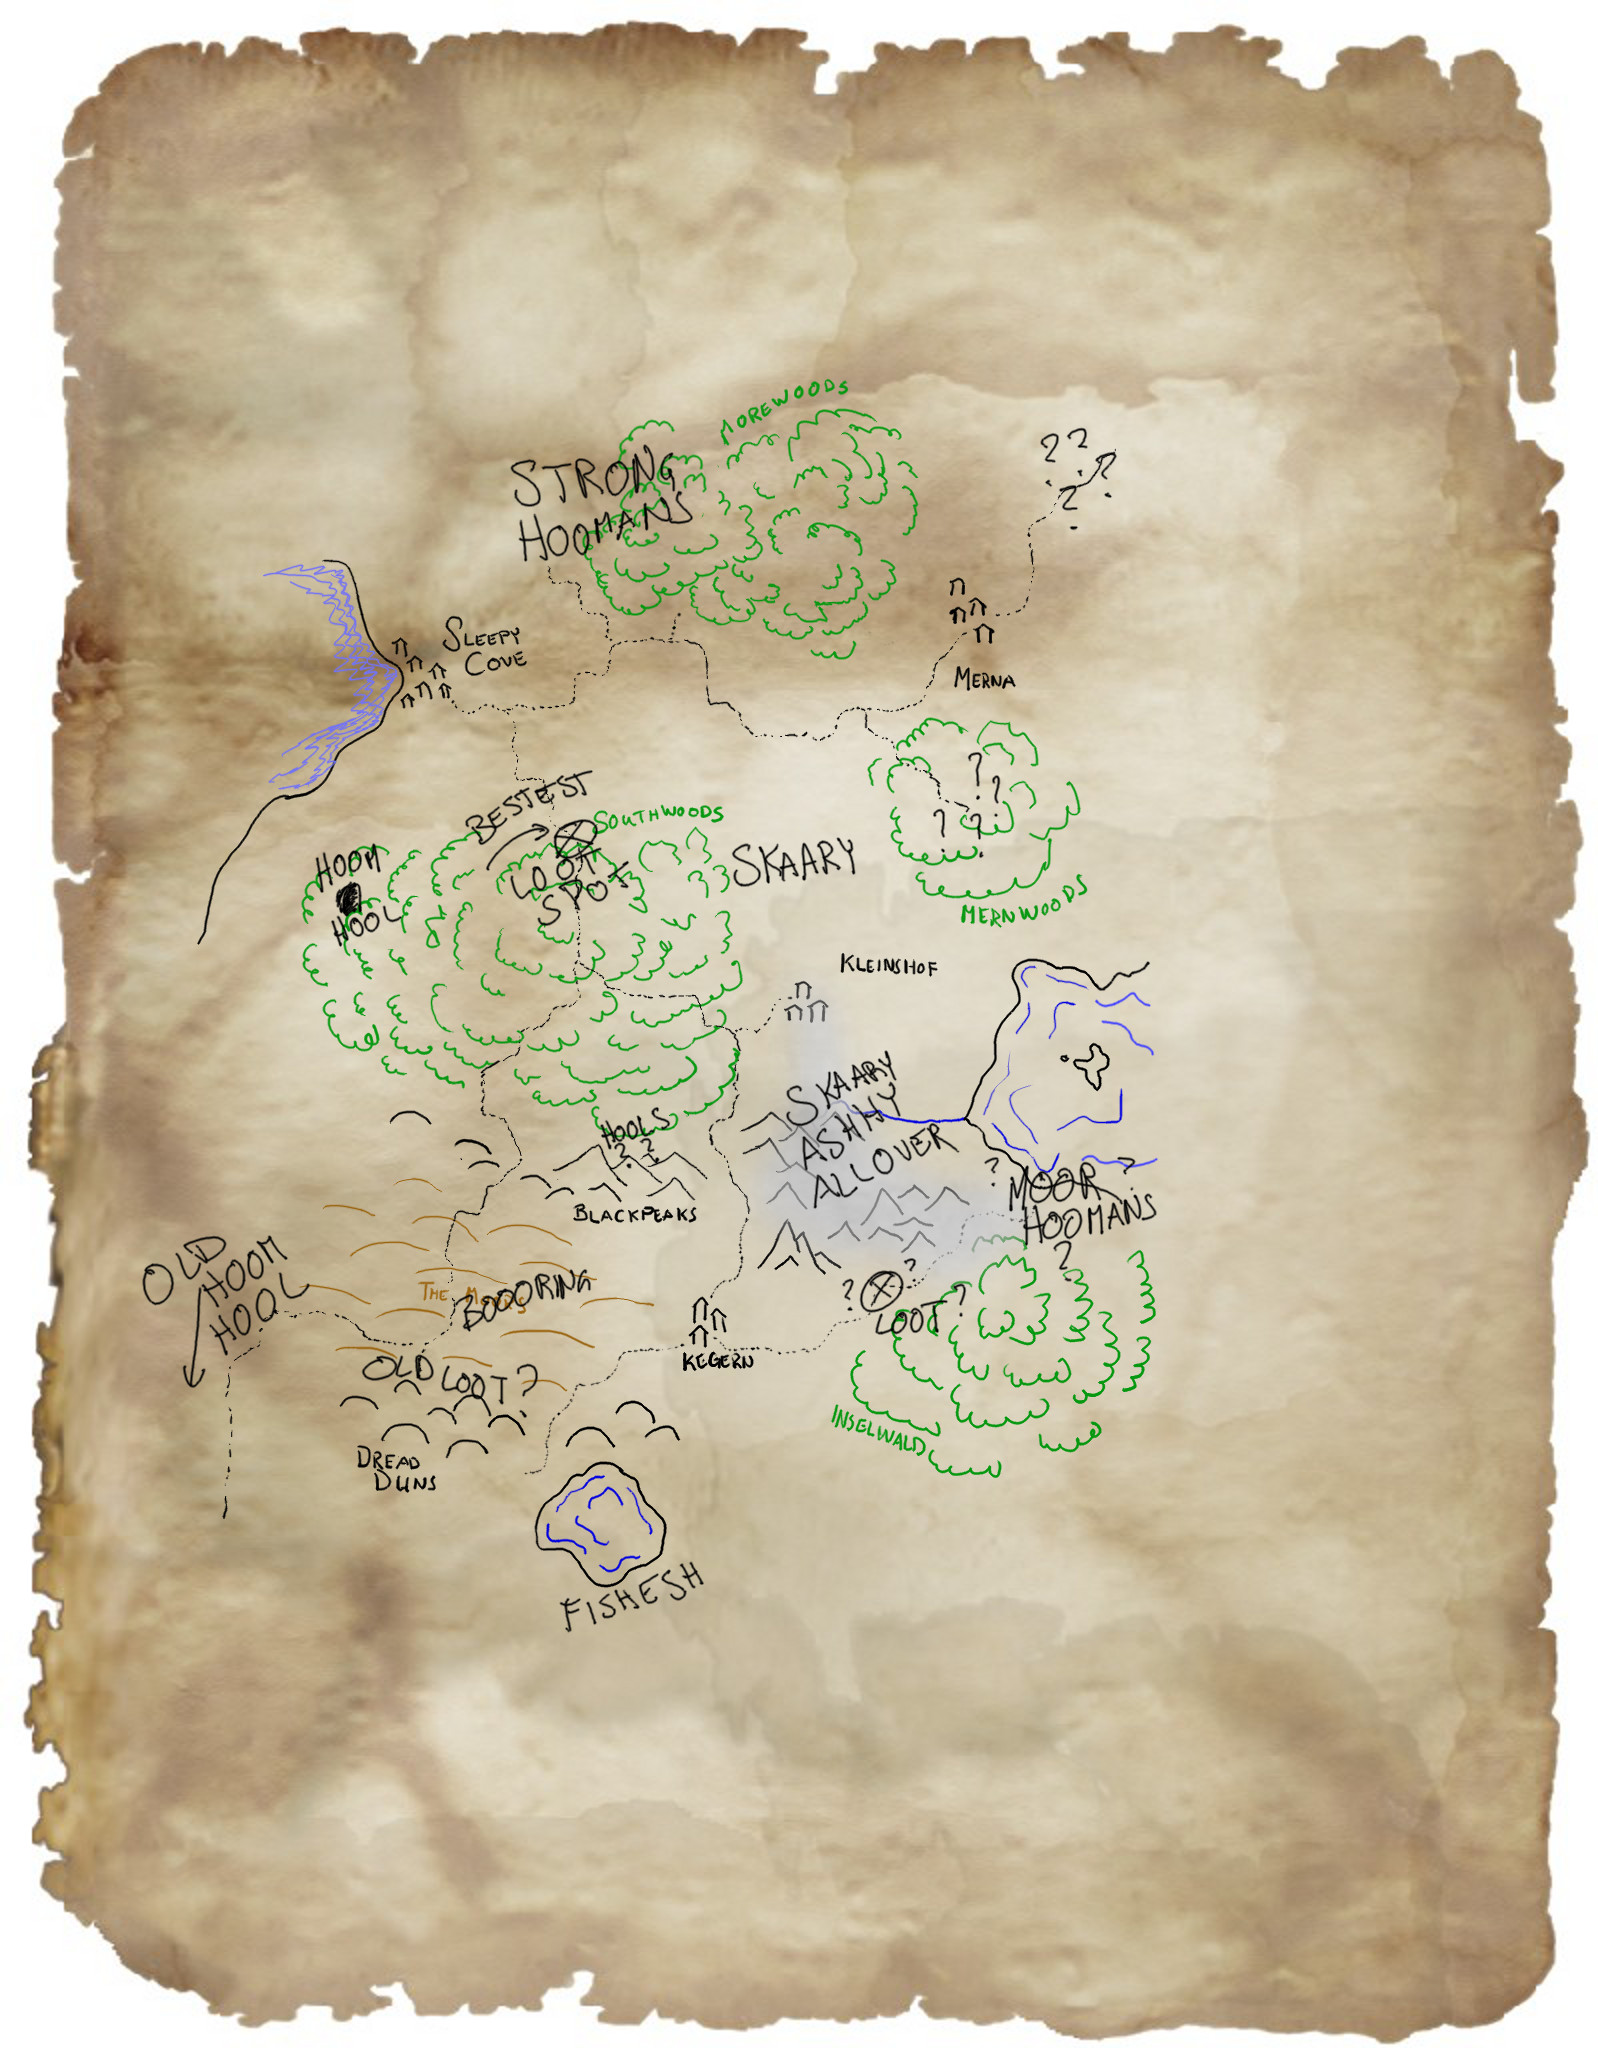
\includegraphics[width=1.0\textwidth]{fig/region.jpg}
  \caption{The local region, as known by GamGang}
\end{figure}

In short: Hoom Hool sits in a rich forest where the gang can forage and hunt for around 50\% of their food. Nearby is a good ambush spot along a trade route from Sleepy Cove harbour to Kleinshof and Kegern. The Gang has settled in and done a couple of quick highway raids at the Bestest Lootspot already. The region map shows what the goblins know of their new surroundings, though nothing outside Hoom Hool, Bestest Lootspot, and their immediate surroundings have been scouted.

The region is under rule of Baron Evilnius Conq. He has light patrols out keeping the peace after the power struggle a while back where he toppled Baron Pawa. There are still some demons and monsters roaming around in the aftermath of the whole Uchly Namen rampage. And then there was this sorcerous plague in the south east which turned the land grey and ashen. Other than that it's a good place to live.

Robert the Reeve is the lawman in charge of keeping the peace around Sleepy Cove, Merna, Kleinshof. He is efficient but selectively corrupt. The Heroes can run into his patrolmen when they travel the wild or visit a village. Any survivors of the goblins' banditry will be screaming bloody murder in Sleepy Cove and Kleinshof and put all patrols on alert for the bandits. If any of the Heroes are particularly memorable in appearance they will be recognised if they enter a village or encounter a patrol, but usually goblins all look alike to humans and people will normally not assume that every bunch of goblins encountered are the Beastly Bandits that the neighbours have been talking about.

Goblins are generally treated well in the region as long as they are part of society; follow the law and don't eat any babies. They are welcome in the villages if they dress well, behave, and try to speak common tongue.

Note that villagers will generally recognise locally stolen property. If the Heroes loot a wagon going from Kleinshof to Sleepy Cove, then try to sell the stuff back in Kleinshof, odds are good someone will notice and call the patrols. The villagers also have a chance to recognise donkeys, wagons, etc originating from the village even if the goods come from somewhere else. Patrol horses, armour, weapons etc are also easily recognisable, leading to questions.
\textit{I swears it! That stupid donkey we took just wandered off to a farm in the village. And woddunt-ya-now, the farmer said it was his, and that we had stole it from him! And then 'em soldiers came runnin'.}

As the goblin banditry escalates Robert the Reeve will send patrols to try to find them. Any survivors might join and help out as well. If Hjalmar Hjälte survives the first fight he will gather survivors and mercenaries on his own, and he is good at tracking the GamGang both to their Hoom Hool and any other camp they might set up in the region. Remember that survivors also get xp, so have them level-up, buy gear, and rent hirelings suitable for revenge.

When it becomes evident that the patrols can't keep the land safe Robert the Reeve will ask Baron Conq to send the Burmak Squad to root out the Goblin Bandits. If they fail the task will go to Captain Lundqvist to take care of the problem once and for all. GamGang might beat Burmak, but should not be able to beat Lundqvist. Scale the encounters accordingly. Lundqvist will drive them out of their lair, forcing them to flee and find a new place to live. And if Lundqvist fails he will come back later with a stronger force.

The Black Peak hools might work if they kill or assimilate the goblin bands there. The old Edwin Chromophobe dungeon should be mostly empty? A forest camp in Mernwoods or the old tower ruin in the Morewoods perhaps? The old ruin on the Moors can work, but orc bands will come and fight them for it. They could even try to live out of the old torture dungeon in the Dread Duns.

As the goblins ambush, raid, pillage, etc throughout the land they will become known. And the people in the villages will learn what they look like.  Patrols will flee and call for reinforcements, the villages will be armed and manned.

Things will get progressively worse and worse, until it's time to wrap up the campaign. Start having GammelTant scare them with GrimGnash horror stories as soon as they come back from fighting SturSkurk. Have scout groups and foraging parties disappear. Then finally, if they don't gather courage themselves, GammelTant will force them to go find GrimGnash and try to kill him. Where they will certainly fail, ending the campaign.


\subsection*{General path through the campaign}

First get the players accustomed to their new goblins by having a couple of robbery fights. "Another Day in the Office" and "Robbery Gone Wrong" introduce Hjalmar Hjälte and SturSkurk, and set the Dread Prophecy of \emph{Death by GrimGnash} rolling.

As time goes on the GamGang becomes more known in the region, more patrols and more caravan guards show up. Villagers have a higher chance of recognising the Villaneous Goblins making trade harder. Hjalmar Hjälte, if surviving, will lead the early attempts to find and hunt down the Goblins. He gathers survivors, patrolmen, hirelings, etc into militia or posse groups.

GammelTant will push for Revenge against SturSkurk. Sooner or later the Heroes will have to go kill him.

After a while the Law of the Land will send specialty squads like Burmak and Lundqvist to combat the bandits. They will likely attack Hoom Hool, but might also follow up on patrol or caravan sightings and ambush in the open or other adventure locations. Burmak will be difficult but beatable. The only way to survive Lundqvist is to flee. Lundqvist and his men will never give up. Even if the Heroes survive an encounter with his force he will get more men and track them down again and again.

Finally GrimGnash awaits, putting an stop to it all.

\

The players have a lot of choice in what they do and when. Make sure they find the treasure map to the torture dungeon early on. While travelling they will see the IffyGriffs far away. Soon the mutated runts will show up and they can lead the way to the magic stream. Throw in patrols, traders and travellers, etc as suitable. Simple things like going shopping can turn into adventures if someone in town recognises stolen merchandise or goblin bandits, perhaps a patrol group is resting at the local inn? A village might hire some warriors to clear the bandits or guard the town or caravans. The Heroes might get tired of GammelTant. Let them try to seize power.

Regardless, get them to attempt an attack on SturSkurk before 150xp. Send Burmak at them before 250xp. Lundqvist should make a first attack before 350xp. GrimGnash before 500xp.

\

The appendices holds a couple of warrior band suggestions. Also look to the previous campaigns in the region for inspiration. If the goblins become too strong perhaps some old player PCs can be used to form an NPC hunting squad against the goblins? Or perhaps Bling Swordslash or Sam Slick?








\clearpage
%--------|---------|---------|---------|---------|---------|---------|---------|
%       10        20        30        40        50        60        70        80
%-------------------------------------------------------------------------------
\phantomsection\addcontentsline{toc}{section}{00 just another day at the office}
\section*{00 just another day at the office}
\markboth{just another day}{just another day}

This is a simple intro fight to get the Heroes tested out, so it's business as usual. Go to the twisty bit of the road and wait for the wagons. Capture some loot and get rich. Cook a tasty Victory Stew from the corpse of an unfortunate farmer.


\subsection*{synopsis}

Travel to the Bestest Loot Spot, set up an ambush, fight the wagon train. Probably get at least some loot even though most of the opposition will escape. Go home and celebrate.


\subsection*{adventure}

Gamling sends the Heroes to do a robbery on their own. They cannot bring any other goblins, wolves, etc from the camp. The Heroes have to fight as they are rolled up and with their starting gear.

\begin{readoutloud}
\emph{[Gamling speaks:]}
Yoo faitas! Yoo go hunt food! We hungry! Me Bizzi! Run get loot at Bestest Lootspot.
\end{readoutloud}

\noindent The Heroes can pick up some minor equipment from the camp, but not much of value. They can't go buying anything new before this first mission either. If they want to bring something of value from the camp have them argue with Gamling about it. Haggle, Leader, or any fancy intelligence based arguments won't work since Gamling will just smack them with superior strength and fighting skills. Instead have a psy-vs-psy nagging argument modified mod-1 for every 10c value they want to bring. If they fail-3 then Gamling will smack the arguing Hero until he shuts up, doing 1hp damage per nag roll. If the Heroes are cheeky and want to roll for defence, allow them at mod=0, just regular light brawling, but if they succeed Gamling gets angry and will try to smack them harder, actually landing a real brawling fist attack. Continue until they give up or flee and stay away for at least a few hours. Or, why not have a tiny fight? Impromptu 1v1 with lots of others cheering on? Gamling won't kill anyone on purpose though. Ganging up on Gamling will bring the whole clan down on them and it will be time to roll new Heroes.

The camp has only a few days worth of food, some torches, a few extra knives, staffs, clubs, shitty spears, rusty axes, goblin short bows, etc. A few hides, some rope, a handful of torches, and other simple equipment is also available. Most of the camp gear is mod-1 or 66\% abs or some such. It's good if they bring the camp's old donkey though, since it can carry a lot more loot than the Heroes can. But let them think of it themselves. Gamling will scream at them when they get back if they forgot it. GammelTant will kill and cook one of them if they loose the donkey though.

The wagons only move during the day so no use bringing night fighting gear. They can of course be sneaky and try to seek out the wagons during the night if they want. They need enough track skill or actually move the party onto the wagon night camp to find it. The wagons travel from Kleinshof to Sleepy Cove, which at 10 leagues per day (10sq/d) takes two days. They camp for the night just north of the trail fork. A lightly forested area with a wagon circle and tents, fire pit, lookout, etc.

Have the players set up the robbery as they please. They have plenty of time to prepare. If any of them pass int rolls you can helpfully suggest things like: \emph{If you'd had anyone with the skill "traps" you could have set traps by the road...}

When the players are finished, start the fight by having the wagon train move onto the map, wagon by wagon over a few rounds. Hjalmar Hjälte leads the train, walking a few squares in front of the first wagon.


\subsection*{map mechanics}

The route along the road is almost 100sq long. Assume the wagons moves at a safe 5sq/r (slow run) after being attacked. That gives 20r for the GamGang to force them to stop before they leave the map.

One way to get more time is to barricade the road with a tree, stones, angry goblins, etc. They can also try to break one of the wagons, or kill a donkey to have the wagon stop at a difficult to pass spot, or some such. But don't hint at them to barricade the road. More fun if they for example have a running fight, chasing the wagons through the map.

The wagons enter the map at speed 3, with 3-6sq empty space between them. Then accelerate to speed 5 when in a fight. The wagoneers and heroes have mod-3 to their perception rolls unless something indicates that there might be an attack incoming. Things like a tree felled over the road will indicate an attack and make them suspicious and careful. Same if they find goblins hiding or in plain sight.

The map has trees, bushes, boulders, etc. Should be plenty of good opportunity to hide, setup an ambush, take cover, etc.


\subsection*{opposition: wagons and Hjalmar Hjälte}

Stats for Hjalmar Hjälte is available in the \hyperref[hjalmarhjalte]{appendix} page \pageref{hjalmarhjalte}. Get stats for typical farmers, swordsman, archers from the rulebook, campaign section. Farmers ca 100xp, swordsmen and archers ca 150xp.

The caravan is led by Hjalmar Hjälte, a not too difficult hero, and guarded by Swordsmen (150xp) and Archers (150xp). Each wagon is driven by a farmer armed with knife or axe and each wagon has either a Swordsman or Archer walking alongside or riding in it.

Hjalmar Hjälte and one wagon should be enough to go against four goblins, then bring in another wagon for every two additional goblins. Recommend first two wagons have swordsmen, then one with an archer, then another archer or swordsman.

The wagons can go faster than 5sq/r but risk breaking down. For every speed step above 5 a wagon suffers 5\% chance per round to loose a wheel, overturn, etc. E.g. at speed 9 it's a 20\% chance per round.

If the road is blocked they will go into defensive position bringing the wagons together, phalanx fighters with archer support, etc. If the Heroes wait to attack (must pass psy or int rolls, goblins are impatient) the farmers will finally act to remove a road block or impediment, but will be guarded by the swordsmen and Hjalmar Hjälte.

If the farmers are loosing and can flee they will dump some loot and no longer suffer the risk of breaking their wagons when they go fast. Without loot a wagon can safely travel 10sq/r and the farmers are great drivers.

Hjalmar Hjälte will make simple attempts to coordinate with the swordsmen guards, and possibly the farmers, but nothing super clever. He will retreat and quaff if hurt. If he still can't win he will flee when almost dead.

Story-wise the best outcome is if Hjalmar Hjälte manages to flee together with some wagons. Then it's natural that he starts trying to gather a posse to go after the goblins a little bit later in the campaign.


\subsection*{loot}

The wagons have mostly food, simple materials, etc. Assume each wagon has total loot for around 10s, but nothing fancy. Just look through the price/equipment lists and pick a few items. E.g: 50x days food, 2x 10l kegs of beer, 6x blankets.\\
Each farmer has 1d3 silver and 1d10 copper.\\
Swordsmen and archers have 1d5 silver and 1d20 copper.\\
Hjalmar Hjälte have 3+1d5 silver and 10+1d30 copper.\\
Also nice if one of the wagons have a hidden bag of 10-20 silver (find mod+3 if they say they search the wagon and spend a few rounds, perception is not enough).

The donkeys are difficult to subdue since they don't like goblins. Requires a series of str vs str successes, or a smaller series of ride successes, or an animal command success per donkey. 

If they bring wagons when leaving it's slow going. The wagons only have 2 leagues cruise speed through forest, and require a successful ride roll per day to avoid getting stuck or damaged by terrain if not on roads.

The loot cannot be sold in Kleinshof since that's where it comes from. The wagons or donkeys cannot be sold in Kleinshof, Sleepy Cove or Kegern. The villagers will recognise the donkeys or wagons and have Conq Solders arrest the Heroes for thievery! Interesting little side adventure if they try.

Note that Gamling and GammelTant will take any money and loot not hidden away and put it to the Coffer. The players should figure out their stories beforehand if they want to sneak something past the loot collector when they return, or they all have to pass int rolls to not let something slip and squeal. This will be the same for the return of every adventure as long as Gamling or GammelTant are alive.








\clearpage
%--------|---------|---------|---------|---------|---------|---------|---------|
%       10        20        30        40        50        60        70        80
%-------------------------------------------------------------------------------
\phantomsection\addcontentsline{toc}{section}{01 robbery gone wrong}
\section*{01 robbery gone wrong}
\markboth{robbery gone wrong}{robbery gone wrong}

Business as usual. Go to Bestest Lootspot and wait for the wagons. Capture some loot and get rich. The problem is that the SturSkurk gang shows up and Gamling gets killed. This is the start of \emph{Goblin Destiny: Death by GrimGnash}.


\subsection*{synopsis}

GamGang prepares a highway robbery. The wagon train enters and the fight starts. Soon the SturSkurk Gang enters the map. Gamling charges SturSkurk Boss and quickly dies. Rest of GamGang flee the fight soon thereafter, grabbing minor loot. It is unlikely but not impossible to beat both the wagon train and the SturSkurk Gang.


\subsection*{adventure}

The food from the previous raid is gone, and the GamGang is starving again. Must have more food! More Loot! This time Gamling himself will lead the outing.

\begin{readoutloud}
\emph{[Gamling speaks:]}
Em faitas! We go hunt moar loot stuff! Grabba em spearsanswords! Hurtysticks for all! Waik em shootas. To e twisty bit we go. Tiny Looka has seen beeg wagon komma! Lotsa loot! Go! Go!
\end{readoutloud}

\noindent Since Gamling is with them they can also add some support goblins. A couple of disposable warriors or fighters, as long as they can all travel fast enough on the region map. The camp is soon hungry again! Gamling will allow at most five days away: two days to Bestest Lootspot, one day for the robbery, two days home again. This means a minimum of four leagues per day. Any goblins who can't keep up should buy "travel" or suffer as Gamling will force march the group. Every lacking league gives the slow-poke 1hp damage and max stamina -1 until home again and rested.

Allow the players to position and prepare for the robbery. But it can't be too clever or Gamling will scream at them to do it differently.

The wagons arrive and there is some fighting, the heavy wagoneer should be an issue. Keep Gamling somewhat near the map border where you plan to have SturSkurk enter. Once SturSkurk arrives Gamling will charge him and die quickly. After Gamling dies SturSkurk will fight both the goblins and the wagon train. The goblins are more of a threat so SturSkurk will focus on them first, unless it costs them loot opportunity.
GamGang should be forced to flee soon after Gamling is slain. Perhaps they pick up some loot along the way.


\subsection*{map mechanics}

Same as before, see the map mechanics section under the previous adventure. But this time Hjalmar Hjälte is not with them even if he survived the last encounter. Instead the wagon train has the heavy Wagoneer at the end. His armoured-illers can clear road blocks to some extent and push carts or bandits out of the way to allow for escape.

As soon as the fight with the wagons has started properly the SturSkurk Gang will arrive. Gamling charges SturSkurk and his two orcs. Make sure Gamling dies in a couple of rounds. Gamling won't defend, just attack all out with his axe. SturSkurk will play it safe and


\subsection*{opposition}

With first the farmers and Wagoneer, then the SturSkurk Gang, it is unlikely that the Goblins will win this fight. Try to balance so that the players feel it really is \emph{very dangerous but not impossible} to beat both the wagon train and SturSkurk Gang. It is possible to get the SturSkurk Gang to fight the wagon train, and carefully pick off some of the people on both sides until the rest of GamGang has a chance to win.


\subsection*{opposition: wagons}

The heavy Wagoneer counts for 2x goblins. For every further 2x goblins add another wagon with guard. Use archer guards and get the farmers to escape as soon as possible.

The heavy Wagoneer comes last in the wagon train. If the road is blocked his armoured-illers can push aside other wagons, or perhaps even a tree if they have some time. The Wagoneer will fight if necessary, but will try to just escape.

The farmers will try to escape, including turn around if it seems to help. Archers can fire from wagons with mod-3.


\subsection*{opposition: SturSkurk}

The SturSkurk gang enters the map in staggered group. Main melee line phalanx, the witch in between, then archers group behind.
They will start to attack the goblins, but will also attack farmers and the Wagoneer if they can snag some loot.

SturSkurk will fight and kill Gamling first, since Gamling will charge him immediately on arrival. The melee phalanx line will protect their archers, and only push into the fight if their archers are not strong enough to win a shooting duel.

Main melee front line is SturSkurk Boss with the two orcs on either side. They move together and fight defensively, primarily mainly making sure that the opposition get pinned in place so their archers can whittle down the outliers. When Gamling charges Boss will block with shield and let the orcs stick him to death. If Gamling leave an opening SturSkurk will 

The Witch will shock bolt and cast slow on Heroes when possible to aid her melee line. She will also run up and use ward shield on the boss and orcs if necessary. Defensively she'll use fire storm.

The SturSkurk archer group will run around to stay out of reach and pepper arrows when possible to suppress Heroes' archers and casters.

If it's obvious that they will loose then Boss will order a retreat.


\subsection*{loot}

The regular farmer carts have similar loot as in "00 just another day in the office", ca 10s worth of food and simple items.\\
The heavy wagon has 100+1d100 days' food, ca 20s of random trade stuff, and a couple of high end items e.g. Quaff!. The wagon is a small camping house and also has a small stove, some cooking gear, a few days of food, minor trinkets, clothes, etc. In a \emph{hidden compartment} in the wagon is 20+1d10 silver and 50+1d50 copper (find roll required mod-0, can't find with perception roll).\\
SturSkurk people have just 1d3s + 1d10c each. Their gear is in ok condition.

Award ca 15xp each for the adventure, and shared xp for the defeated opposition. Don't deduct if the Heroes flee. They are supposed to run away here. Add another 5xp each if they force SturSkurk to flee.






\vfill
%-------------------------------------------------------------------------------
\section*{Gamling is Dead, all hail GammelTant!}

After Gamling has died GammelTant will be furious for a bit, call for revenge, and send Hemskelina to scout for the SturSkurk gang. Soon she remembers the Old Prophecy of \emph{Death by GrimGnash}, and locks herself away with her crystal ball.

When Hemskelina comes back reporting of the SturSkurk bandit camp location GammelTant immediately sends out the Heroes to kill them all and steal all their shit. And of course to bring back the corpse of the Blue Boss so she can cook a Victory Revenge Stew!










\clearpage
%--------|---------|---------|---------|---------|---------|---------|---------|
%       10        20        30        40        50        60        70        80
%-------------------------------------------------------------------------------
\phantomsection\addcontentsline{toc}{section}{02 kill the bandits}
\section*{02 kill the bandits}
\markboth{kill the bandits}{kill the bandits}

The camp of the SturSkurk bandits has been found and scouted by Hemskelina. It's time to kill them all! And eat the good ones.


\subsection*{synopsis}

Kill the SturSkurk bandit gang by assaulting their camp. Best to assault at night. Scout the camp perhaps. If fail -- try again later on.


\subsection*{adventure}

The Heroes are in control of the planning. Hemskelina is coming along but will not fight as a lead figure. Her task is to kill Blue Boss if he tries to escape.
The Heroes can bring a couple of fighters, warriors, runts, and a wolf if they want.

\begin{readoutloud}
\emph{[GammelTant shouts:]}
Go Get Em Killt! Blue Boss bring back! Kook-em corpse in Victory Revenge Stew I will! Take-a em few warrjas and fajtas with-ya!
\end{readoutloud}

\noindent The Heroes can position and prepare for the camp assault but they cannot dig trap pits or do similar heavy work/noise activities in the area without getting spotted.

Hemskelina will have scouted the outskirts of the camp but not the interior. Provide limited view into the camp from a few vantage points. The Heroes can see the outline of the camp but not all of the the interior.

SturSkurk gang will have a competent scout on guard patrolling the camp. Hemskelina will track him but need help to kill him quickly.

\

This should be a tough fight. The Heroes might fail their first attack and have to come back later with a better plan or some help.
A clever idea could be to go to one of the villages nearby and talk to a patrol soldier about "this nasty bandit gang in the forest camp over there" and have the soldiers fight SturSkurk. But SturSkurk is also somewhat smart, he has already bribed the patrol captain in charge of the region between Sleepy Cove and Kleinshof. For this to work the Heroes must go further North to Baron Conq's castle up in "Strong Hoomans" territory and talk directly to the
\textbf{TODO finish this} talk with military leader, only if not already known, before Burmak attack, before any patrolmen have escaped fights,



\subsection*{map mechanics}

Apart from a couple of guards the bandits are sleeping hidden in their tents and their icons should be hidden completely until they step out of the tent or someone peeks into the tents.

\small \begin{verbatim}
bla bla bla
\end{verbatim} \normalsize


\subsection*{opposition}

bla bla bla


\subsection*{loot}

bla bla bla


\subsection*{playthrough}

bla bla bla







\clearpage
%--------|---------|---------|---------|---------|---------|---------|---------|
%       10        20        30        40        50        60        70        80
%-------------------------------------------------------------------------------
\phantomsection\addcontentsline{toc}{section}{03 defend hoom-hool}
\section*{03 defend hoom-hool}
\markboth{defend hoom-hool}{defend hoom-hool}



\subsection*{synopsis}

The Law of the Land attacks Hoom-Hool to drive out the Goblin Scourge. The Heroes barely survive and some attackers flee.


\subsection*{adventure}

Most likely this will happen once or twice. Perhaps a surviving Hjalmar Hjälte gathers a possee and make a doomed attempt to take revenge on the Goblins. This should be beatable without too heavy losses.
Later on Burmak will attack. This is supposed to be difficult but the Heroes should win.
For Burmak and six spear men and Hjalmar Hjälte alive from before it's recommended that the Heroes have ca eight goblins at ca 130xp each, along with Hemskelina, GammelTant, some warriors and fighters, and some runts.
If the Heroes flee and are forced to relocate here then skip the Lundqvist attack in "04 flee and relocate".

\begin{readoutloud}
\emph{[SomeDude speaks:]}
Go Get Shit Done!
\end{readoutloud}

\noindent bla bla bla


\subsection*{map mechanics}

With them are any survivors from the "00 just another day in the office", and perhaps a couple of experienced hirelings.
bla bla bla

\small \begin{verbatim}
bla bla description etc
\end{verbatim} \normalsize


\subsection*{opposition}

bla bla bla


\subsection*{opposition: Burmak Guard Squad}

Guard Captain Burmak and his squad of spear men have been tasked to root out the Goblin Menace. Burmak will keep his men in tight formation, using phalanx and spear reach to attack with a second line. The front line will declare more actions and be defensive, while the back line will declare fewer actions and be offensive over their front line brethren. The back line can also throw javelins.

Burmak will fight from the rear, using his leadership, high initiative, and Oy! to keep his troops fighting in synchronisation and high initiative.

Burmak will call retreat if he gets hurt below 8hp or looses half his men.


\subsection*{opposition: survivors}

The survivors from the "00 just another day in the office" robbery will come along. If Hjalmar Hjälte is with them they will probably lead the charge, and if not they will be behind Burmaks squad.


\subsection*{loot}

The soldiers and survivors don't have much money on them. Their equipment is in good condition though.


\subsection*{playthrough}

bla bla bla









\clearpage
%--------|---------|---------|---------|---------|---------|---------|---------|
%       10        20        30        40        50        60        70        80
%-------------------------------------------------------------------------------
\phantomsection\addcontentsline{toc}{section}{04 flee and relocate}
\section*{04 flee and relocate}
\markboth{flee and relocate}{flee and relocate}


Another attack on Hoom-Hool. This time Lundqvist Soldier Squad will force the GamGang to flee and relocate.


\subsection*{synopsis}

The over powered Lundqvist squad will be too difficult for the GamGang goblins and they will have to flee.


\subsection*{adventure}

The people of Kleinshof and Sleepy Cove have finally managed to get a local lord (Conq?) to send out a proper military group to root out the Goblin Menace hiding in the woods.

\begin{readoutloud}
\emph{[SomeDude speaks:]}
Go Get Shit Done!
\end{readoutloud}

\noindent bla bla bla

\subsection*{map mechanics}

bla bla bla

\small \begin{verbatim}
bla bla description etc
\end{verbatim} \normalsize


\subsection*{opposition}

bla bla bla


\subsection*{loot}

bla bla bla


\subsection*{playthrough}

bla bla bla










\clearpage
%--------|---------|---------|---------|---------|---------|---------|---------|
%       10        20        30        40        50        60        70        80
%-------------------------------------------------------------------------------
\phantomsection\addcontentsline{toc}{section}{05 Death by GrimGnash}
\section*{05 Death by GrimGnash}
\markboth{GrimGnash}{GrimGnash}


The prophecy comes true. Death by GrimGnash. No way around it. Here ends the campaign.


\subsection*{synopsis}

Either they go hunt down GrimGnash where he sleeps in his lair, or GrimGnash attacks them somewhere else. Either way most die, some might flee to survive. If they try to attack then flee GrimGnash will find them and attack elsewhere very soon.


\subsection*{adventure}

GammelTant, or whoever is the leader at the time, sees Certain Death each night in the crystal ball and feverish nightmares. Huge Teeth and Claws rip the goblins apart. No matter where they move the Teeth and Claws come hunting for them.

\begin{readoutloud}
\emph{[GammelTant:]} Mussst go kill GrimGnash! Or it comes Kill Us All! Find it sleeping and Slay it Dead! Deader! Deadedd for sure!
\end{readoutloud}

\noindent GrimGnash sleeps in his lair in the high peak above the clouds. Best if the goblins find the lair and then attack when GrimGnash is asleep. GrimGnash can always attack them at any open sky map, flying over again and again torching them and whatever else can burn on their local battle map to crispy death and ash.

When he sleeps they can enter his lair and make some sort of clever attack. He will of course wake up and start killing the intruders.


\subsection*{map mechanics}

The map is split by a bottomless chasm. The walls can be climbed at mod+3. The platforms are elevated but not high and can be climbed in 1r at mod+3 or jumped in 3ap with \emph{both} successful acrobatics mod-3 and dex+jump mod-3 rolls. 

The large northen fire pyres look different. Something is odd. When close (within per sq), roll per to notice that they look like they are alive and writhing. 
\begin{readoutloud}
The fire burning in the large pyres looks unpleasantly strange, flames moving around like they have a life of their own.
\end{readoutloud}
Casting ranged spells within the cave will spawn a fire elemental from one of the large pyre vats on the north section. Each pyre vat can spawn one elemental per round.


\subsection*{opposition}

GrimGnash himself and a bunch of Fire Elementals that can spawn from the two large pyres in the north section of the map.

GrimGnash is a colossal (6x6) size monster with lots of hitpoints and thick scales, claws, teeth, tail, and fire breath. He's fast and can fly. At low hp he will regenerate slowly. He'll focus on high damage dealers and either swat them away or try to grab them and bite their head off. For multiple grouped attackers he will use fire breath or tail swipe. If in danger he'll fly to safety or simply rush through enemies throwing them aside.

Fire Elementals are simple. They will swarm targets and coordinate movement and attacks somewhat intelligently. They can move unhindered up and down platform edges.


\subsection*{loot}

GrimGnash is rich, but he's also really vain. He's been spending most of his gold on giant skeletons, fake treasure, large magic pyre vats, huge intimidating torches, etc. So there's not so much actual gold left, not compared to how the cave is decorated.

There is a treasure chest hidden in a niche in the north wall. Roll find+3 if searching the area, or per-6 if walking by when looking for loot.

All over the northern dias is a huge pile of treasure. Closer inspection will show that it's all fake treasure.

All weapons found in the lair are of good quality, but enormous. They have never been used and are polished weekly. Assume 4x normal abs, requiring 10 + 2x normal strength, and suitably high damage potential. The scorched skeletons are well maintained and carefully posed, and from enormous giants, 3-5m tall.


\subsection*{playthrough}

bla bla bla












\clearpage
%--------|---------|---------|---------|---------|---------|---------|---------|
%       10        20        30        40        50        60        70        80
%-------------------------------------------------------------------------------
\phantomsection\addcontentsline{toc}{section}{XX patrols}
\section*{XX intermission: patrols}
\markboth{patrols}{patrols}


Patrols from the Castles or villages travel the lands to search for enemies, hunt bandits, and safeguard routes for travellers and merchants. The patrol soldiers are not automatically hostile. All depends on how well the goblins are known, what they do and how they are dressed when meeting, and what they are carrying.


\subsection*{synopsis}

When travelling they run across patrols. Talk or fight. Look and behave like civilians or fight like bandits. Small low level patrols are easy to trick unless anything "bandity" is obvious. They are also not that tricky to fight.


\subsection*{adventure}

Patrols are most likely along the roads, but will be out in the field as well. They usually don't enter the forests unless necessary.

\begin{readoutloud}
\emph{[Friendly Patrol Soldier speaks:]}
Hello hello there! How's life this fine day? Where are you fellows travelling this day? Anything interesting in those wagons? My dear wife is looking for some fine cloth for a new dress. Can you give me good price?
\end{readoutloud}

\noindent The Heroes need to either talk their way through the patrols by pretending to be traders, or bribe them, or fight them. The important part is to not allow any patrolmen on horseback to escape, which will immediately bring more soldiers down on them, as soon as they can get there.

If the goblins can pass for peaceful traders or farmers this is not an issue. If they start fighting and the soldiers are loosing they will try to flee, and one will take off on horseback to get help. Any soldiers that manage to flee will try to follow the goblins at a safe distance (a few leagues behind), but only have limited track (3 or so).

Response groups can be called from Castle Pawa or Castle Conq and can travel up to 15 leagues per day. They will be 5-8 cavalry soldiers and have a scout (track 7) with them. They will likely be very quick to track down the goblins unless they can get into hiding quickly, or are very good at track or sneak to sufficiently hide their tracks.

Civilian militia response groups can be called from any village, but will generally only be farmers, hunters, and a couple of hirelings. They travel at 8 leagues per day, and will have a good hunter (track 9) with them. A civilian militia group will not necessarily attack when they find the goblins. It may be enough that they track and stay nearby, to join with a later real military group.

If a civilian militia is raised from Sleepy Cove and Hjalmar Hjälte is alive, then he will join it together with any other survivors from the previous battles who happen to be available in the village.


\subsection*{map mechanics}

Just open field or plain. Add some rocks and trees, or old ruins, to make the terrain more interesting, but it should be relatively open battle ground.
Encounter will probably be during the day, unless the Heroes see a patrol camp, or the weary solders see the Heroes' camp.


\subsection*{opposition}

Just a small patrol group. One or two on horseback and three to five on foot. The soldiers fight with crossbows at range, one or two salvos, then switch to spear and shield phalanx in close quarters.

They will try to flee if the fight is not going their way, and they will immediately try to send someone on a horse to get help and report once they see that they can't handle the goblins themselves.


\subsection*{loot}

The soldiers' gear is in good order, and they have some coin. A horse or two is also worth quite a bit of money, or food. A civilian militia group has less gear and coin.


\subsection*{playthrough}

This encounter doesn't take much time. We played through one when the GamGang tried to travel to Sleepy Cove to buy food and sell off some loot. The Heroes were horrible at speaking Common so the initial talking was difficult, but then a couple of hot headed goblins started swinging clubs, aaand it was off to the races.

They managed to immediately kill the soldier on horseback first when he tried to make an attack run, and then quickly caught and dispatched the rest of the soldiers with magic (slow, fireball).

20 rounds: r1-10 distance, close, talk, r11-r19 battle










\clearpage
%--------|---------|---------|---------|---------|---------|---------|---------|
%       10        20        30        40        50        60        70        80
%-------------------------------------------------------------------------------
\phantomsection\addcontentsline{toc}{section}{XX mutamonsters}
\section*{XX intermission: mutamonsters}
\markboth{mutamonsters}{mutamonsters}


\subsection*{synopsis}

GamGang discovers a magical stream in the forest. It can turn them into strange mutants and turn weapons magical. They can fight mutated monsters for access. If utilised some chars can get special powers or magical stuff.


\subsection*{adventure}

Either they stumble across this are when travelling through the forest, or they get alerted when two very strange runts show up in their camp. If just happening on the area just put them on the map without any significant intro.

One day two runts come back from a hunt, seriously mutated. One has wings and the other has three arms. They are also somewhat changed mentally. Also, the stone knife carried by one seems to have become magical.

\begin{readoutloud}
The forest is deep and dark, ancient and powerful. No sunlight make it down through the heavy canopy of enormous trees, the forest lies in deep darkness. In the distance you see soft blue-green lights slowly move among the trees. And there is a strange tingly feeling in the air.
\end{readoutloud}

%\noindent bla bla bla


\subsection*{map mechanics}

The map is always a low light area, even in the middle of the day this magical deep forest is always nightly dark.

This is an endless map. More critters will always keep coming, with periods of low population or empty map if the Heroes are fast enough to kill off everything. The surrounding forest spawns light bugs, air fish, moss lumps, and larva. The stream spawns air fish, moss lumps, and tentacle crabs. Stuff trickle in every few rounds, with larger batches every 10-20r, and full synchronised repopulation waves around every 50-100r over a few rounds. New monsters don't immediately start attacking the Heroes. They will meander around for a bit, but get aggressive when attacked, and start to draw others to the fight.

The monsters are aggressive towards non-mutated folk and animals. They ignore mutated people as long as they are not attacked.
Light is an issue. The light bugs are attracted to light sources, and will get aggressive when they find non-mutated folk near a light source or in their own feeble light (2sq or so). The lightbugs will however not fly into major fire, e.g. fire balls, etc.

It's ca 30sq to the magic island if they follow the road, so at least 10 rounds at normal pace, and 3-5r if someone manages to dash there to scout. It's about 20sq straight shoot through the trees, so the island can seen after the first tree, or glimpsed if they explore south a bit.

All the wild magic in the area is refreshing for the goblins. Any goblin heroes (not other races) regain 1 mana and 1 stamina each 10r.

The mutamonsters are also randomly magical. If attempting to drain them they will have 1d10 mana available and 3+1d10 psy for the resistance roll. After 5+1d10r this has "recharged" to a new random amount and protected by new random psy value. It is not possible to push the critters to sleep by draining them to 0 temporary mana.

The first \emph{successful} expedition to the magical light will give full xp for the exploration, kill, and map clearing. If they return again to boost a new character or weapons the map will have repopulated, but will not give any more xp.


\subsection*{opposition}

Mutated monsters: Ranging from very large tentacle crab to tiny explosive light bugs. See the mutamonster appendix for details on the various critters. %TODO set hyperlink

The monsters don't coordinate much, but the light bugs will probably drive people on the move during the fight, or require that a spellcaster keep bolting them. As they move they will stir up and attract more monsters as they go. Once in a fight the violence and smell of blood will quickly attract other mutamonsters.

The mutamonsters don't attack other mutated beings. So the already mutated runts can move freely in the area if they are present. Don't tell the players this though, and see if they notice. The mutated runts don't want to attack the mutamonsters either, so they must be forced to do so. This also applies to mutated Heroes who return to the map later. They won't get attacked until they get aggressive.

Start out with a tentacle crab half in the water near the magic island, and 1-2 larva roaming the forest, along with 5-8 moss humps, 4-6 airfish, and 10-12 light bugs spread out with another 3 near the magic island.
Before the fighting starts the light bugs and airfish lazily amble around 1-2 sq/r, the rest stay mainly still.

As long as the Heroes are in the area new monsters will come from the forest and the stream, random alone and in waves. Keep the players stressed. This is not just a clear out and rest place. It takes fighting and mobility to stay here any significant time. Short respites can be had if they are quick to kill off and clear the map.

If the Heroes flee the map it will rapidly repopulate before they can return.


\subsection*{loot}
%-----------------
Magical Mutationous Powers and Mutamonster Meat awaits those who survive long enough.

Miscellaneous body parts from the mutamonsters can also be sold in the villages at 50\% chance, and shipped to TradeTown for more gold if the Heroes can arrange for it.

If they manage to freeze, sleep, or otherwise capture lightbugs and bring them to the camp, Goblanda will be excited and start cooking up fun stuff. Including detonation grenades in 1d10+5 days, with each lightbug yielding two grenades.


\subsection*{loot: mutamonster meat}
%-----------------------------------
Mutamonster meat is edible but poisonous and with side effects. Eating mutamonster meat should have some fun effects like temporary stat changes, odd roll behaviours, perhaps very temporary abilities or curses. And of course: interesting cosmetic anomalies. Temporary in the beginning, but if the GamGang set up the forest stream as a significant long term food source the oddities should become permanent and they will start to take permanent damage from the weird food.

Aside from fun miscellaneous side effects, all food prepared from mutamonster meat gives temporary psy-3 and for two days. For every week eating high mutamonster meat diet the Hero takes a permanent psy-1 and temporary str-1 and stamina-1. If they keep going the temporary str-1 and stamina-1 will become permanent and cumulative, as will the permanent psy-1.

Make sure to describe the strange effects from the food so the players have a chance to figure things out before it becomes an issue.


\subsection*{loot: magic mutations}
%----------------------------------
Going to the island and touching the magic light has some chance to give serious bodily changes, as well as affect equipment brought there. The longer the Hero stays there, and the more he touches the light, the more mutations he will get. At first it's generally good, then it will become worse and worse. Be careful to describe the effect and give the player a decent chance to figure out that it might be a bad idea to stick around too long. Each "tick", giving a new mutation seed, should take a few rounds to give the player time to think.

\

\noindent Example:
\begin{readoutloud}
Climbing onto the little island you reach out to touch the shimmering light. A sudden spark hits you with a quick stabbing pain \emph{(take 1dam 1pain)}.\\
Suddenly the skin around the strike starts to turn \emph{blue/pink/purple/orange} with discoloured tendrils rapidly growing up your arm onto your body.\\
\emph{E.g: growing a wing:} You feel muscle and bone starts shifting in your back and a small lump growth starts pushing against your armour.\\
\emph{E.g: extra arm:} An itchy crawling feeling in your left armpit... a tiny runt arm is crawling out of an angry red oozing welt.\\
Your mind is reeling from the strangeness \emph{(take psy-1 permanent)}.
\end{readoutloud}

\noindent The first mutation should be something small and cosmetic: big eyes, glowing snot, purple skin, extra big flapping ears, smoking nose, tail, long curly hair, extra fingers, snake tongue (speaking-2, per+1), etc. This first hit gives a psy-1 permanent mod. Successive mutations do not have \emph{this} automatic penalty.

If the Hero stays longer, or touches the light again for a second time, he will get a serious ability. Roll from the list of serious mutations. Initially it will just manifest as a weird lump or similar but will, over time and with xp, grow into whatever is suitable for the ability. An extra arm, smelly pustules, brain nodules, etc.

Remaining in the light longer and repeatedly touching the light will get worse and worse with more detrimental mutations, draining stats, etc. Effects:\\
1st: roll 1x Cosmetic weirdness and 1x Minor boost\\
2nd: roll 1x Serious mutation with suitable cosmetic component\\
3rd: roll 1x Major boost, 1x minor drain\\
4rd: roll 1x Dubious mutation with suitable cosmetic component, 1x minor drain\\
5th: roll 1x Cosmetic weirdness, 1x minor drain\\
all further rolls give 1x minor drain and int-1 or psy-1 (50/50)

\

The mutation seeds will develop over time. If the Heroes don't spend xp on them, let them start stealing some of the xp from each session and start developing on their own anyway.


\raggedbottom

\goodbreak \small \begin{samepage} \begin{verbatim}
Cosmetic weirdness, 1d18:
 1-3   big eyes
 4-5   glowing snot
 6-8   colourful skin: purple/pink/orange/yellow/red
 9-10  polka dots
  11   moving moustache
  12   clattering teeth
13-14  useless tail
15-16  smoking nose
17-18  squeaking knees, sneak-1
\end{verbatim} \end{samepage} \normalsize

\goodbreak \small \begin{samepage} \begin{verbatim}
Minor boosts, 1d13:
 1-3   str +1
 3-6   con +1
 7-8   psy +1
 9-10  hp +1d2
  11   stamina +1
12-13  mana +1d3
\end{verbatim} \end{samepage} \normalsize

\goodbreak \small \begin{samepage} \begin{verbatim}
Major boosts, 1d24
 1-3   str +1d3
  4    dex +1
 5-7   con +1d3
  8    int +1
 9-10  psy +1d3
 11    per +1d3
 12    cha +1
13-16  mana +1d5
17-18  hp +1d5
 19    abs +1
20-22  stamina +1
       vision +1d5 range +1d
23-24  increased size, goblin becomes normal size, str+2, con+2, hp+3
       must eat full rations each day
       re-roll for already full size Heroes
\end{verbatim} \end{samepage} \normalsize

\goodbreak \small \begin{samepage} \begin{verbatim}
Serious mutations, positive, 1d26:
 1-5  Extra Extremity, roll for which below
 6-8  Tasty
 9-11 Foul
12-13 Reactive Skin
   14 Regeneration
   15 Grapple
   16 Incorporeal Double
   17 Teleport
   18 Reach
   19 Blink
20-22 Cockroach
23-24 Black Knight
25-26 Painless
\end{verbatim} \end{samepage} \normalsize

\goodbreak \small \begin{samepage} \begin{verbatim}
Which Extra Extremity, roll 1d10:
1-5  arm: as normal by the ability
6-7  leg: balance+3, r+1, d+2,
          brawl kick: dam+1
8-10 tentacle: climb+3, wrestle+3, block+3
          moves independently up to 2sq from body
          tentacle has 3hp, ranged tohit-6
                            melee pierce tohit-3
          brawl slap: dam 3
          brawl grab: dam 1 pen 2,
                hold: str-3 vs str
                      break free attempts do not cost
                      ap for the tentacled holder
          grows back: on successful con check, 1x/day
\end{verbatim} \end{samepage} \normalsize

\goodbreak \small \begin{samepage} \begin{verbatim}
Dubious mutations, 1d23:
1-3   reduced size (change token size), runts cannot shrink further
      str-1, dex+1, con-1, hp-2, r-1, d-2
4-5   increased size (size +2 steps), goblin becomes 2x2 size,
      2x str,con, 3x hp, r+1, d+2
6     increased size (size +3 steps), goblin becomes 3x3 size,
      3x str, 2x con, 5x hp, w+1, r+2, d+3
7-9   Bulbous Behind: Ever seen a Centaur? This is more of a Dachshund.
      The Hero grows a large derriere, complete with extra legs.
      The "behind" is an extra token that should always be
      placed straight behind the Hero's main token along path
      of movement, hero can still "face" +/- 45deg without
      moving the rear. Moving the rear costs no extra mp.
      r+1, d+2, hp+5, balance+3
10-12 Stone Skin: abs+1, dex-2, cha-3, speaking-3
13-15 Metabolism: stamina+2, must eat 4x full rations each day
16-18 Evil Mini Twin, conjoint: A nasty little malformed mini with an
      evil mind of it's own grows out from the stomach/back/side of
      the Hero. It will sometimes cooperate
      cha-3, hp+2d3, counts as 3enc, has 1d2 tiny arms (str 1d3)
19-23 Glowing: light source range 2d3 -1/abs of armour,
      will attract monsters like "tasty"
\end{verbatim} \end{samepage} \normalsize

\flushbottom


\subsection*{loot: magifying gear}
%---------------------------------
Bringing items and leaving them on the island for a few days will make them magical, for better or worse. It's a 50/50 chance the items will just disappear, or get destroyed. If they remain, then they accrue some fun minor behavioural hiccup, boost, defect, or cosmetic change.

Examples: colour change, glowing, smoking, hot, cold, burning, dripping water, attack+1, parry+1, reach+1, knockback+1, abs+/-50\% or even +100\%, or "indestructible", wielder stat changes like str+1 or int-1, or giving special ability like "Black Knight 2" or "Combat Advantage", or simply tagged "magical" meaning it can harm some incorporeal things and special monsters.
Perhaps the weapon seems to be cool with a mod+1, but actually gives 50\% of failing all hits that are not success+3 or better? A sneaky curse.


\subsection*{playthrough}
%------------------------
The players decide to go hunting for a new Hoom Hool after they hear from a patrol that Hjalmar Hjälte is searching for people to form a posse to go root out the Evil Goblin menace he thinks have settled in the old Goblin Cave in the west of SouthWoods. GammelTant is against the idea since they have defeated Hjalmar Hjälte before, but since she has enough food for a little while she doesn't care much.

Opposition balance: The players initially brought 8 goblins around 130-140xp.\\ Approximated critters: initial : 12 bugs, 4 fish, 6 lumps, 2 larva, 1 crab, spread out and not attacking in coordinated fashion.\\
Goblin reinforcements for following sessions: 3x more goblins\\
Critter spawns: 8 bugs, 3 fish, 4 lumps, staggered spread.

Fighting for 39 rounds. Almost killed 3 goblins, wounded 2 more, all got down to zero mana, most around 0 stamina.\\
Played the critters in an uncoordinated fashion, with no tactical deviousness. The players could quickly see the behaviour patterns and start planning and coordinating their side of the fight.

\

Session 1: rounds 1-3 explore, 4-13 fight, 2h30m\\
They travel towards BlackPeak Mountains, and have trained a few points of "track", so they actually notice when they pass close to the forest stream map marker.\\
On map they start exploring, run into exploding bugs, quickly realise the problem and change tactics. Start bolting bugs. Get stuck hammering away at moss lumps, fish and more lumps are attracted with staggered arrival. Goblins manage to control positioning and have the control of the fight until one of the larva joins in and wrecks their strategy.\\
One goblin gets seriously wounded and has to flee the fight.

\

Session 2: rounds 14-23 fight, 2h45m\\
They bring in one very quick melee rapier goblin to the fight. The larva is tricky until they can re-position their fighters for better efficiency against the heavy armoured grub and bring spear wielders to the right positions. Once they have figured out the details they immediately handle the arrival of the second larva in a quicker more efficient way, but still have problem with positioning since the heavy larva can tackle and force them out of the way easily.\\
In the end their spell casters have near zero mana, and most fighters have very low stamina.

\

Session 3: rounds 24-28 fight, 29-31 cleanup, 32-39 crab, 2h55m\\
They bring in 2x new heavy 2h club melee goblins. They kill off the second larva and the staggered reinforcements very efficiently now that they know the monster behaviour and weaknesses. They mop up the last critters, almost clearing the map, and can rest for a couple of rounds as they advance on the crab. The crab fight is relatively quick since they can bring in the heavy melee club wielders in the forefront, though one of them almost dies and the other gets seriously wounded.

\

Session 4: rounds 29-55 just a quick cleanup and then the goblins swarm the island to fiddle with the magical light while keeping occasional monsters at bay. They are surprisingly cautious and don't stay long. A couple of ability seeds get mutated into a few of them but most just get the small boost and weird cosmetics.










\clearpage
%--------|---------|---------|---------|---------|---------|---------|---------|
%       10        20        30        40        50        60        70        80
%-------------------------------------------------------------------------------
\phantomsection\addcontentsline{toc}{section}{XX iffygriff eggs}
\section*{XX intermission: iffygriff eggs}
\markboth{iffygriff eggs}{iffygriff eggs}


Just a small side adventure, should come somewhat early in the campaign. Save it for an evening when only a few players are available.


\subsection*{synopsis}

Iffygriffs have been spotted flying to and from The Moors. IffyGriff Eggs are a delicacy for the goblins...


\subsection*{adventure}

They have seen IffyGriffs and go scouting for the nest. They want to get the eggs which are a delicacy to goblins. The eggs are also worth quite a bit of money if they can be brought quickly to a larger town.

\begin{readoutloud}
\emph{[GammelTant roars:]}
Go Get Me Em Eggs! Or I Will Make Goblin Cook Stew For Next Dinner!
\end{readoutloud}

\noindent Travel south to the moors. They'll need some track skill to easily find the iffygriff nest site.

The IffyGriffs live in the ruined tower. The other tower has somewhat intact roof and walls and it is possible to hide in there, but the roof and walls are very unsafe and might collapse if an adult iffygriff attacks.

If the goblins arrive in the day at least one adult iffygriff is away hunting. At night both adults are present.

The small bandit gang is present on a 50/50 basis. Adapt to suit the level and amount of Heroes. Can also switch out goblins to heavier orcs. The bandits have smeared iffygriff poo over themselves to not get attacked by the birds. \emph{This works, but will eventually eat away at their armour, then clothes and skin, highly toxic.}


\subsection*{map mechanics}

The IffyGriffs are housing their nest in an old crumbled tower ruin. There is no roof and a sturdy tree growing in the old ruin.

The ghost in the western tower activates when someone enters the tower. It only speaks Ancient. It will ask all who enter (in ancient):
\begin{readoutloud}
\emph{[ghostly whisper (in ancient):]}
Have you come to relieve me and take up my post?
\end{readoutloud}
\noindent If they can't understand, or don't answer (in ancient) that they will take up his post he will scream \emph{Intruders!} (in ancient) and attack. The scream is a fear attack with: fear mod-3, on fail: flee and drain 3stam 3mana, fail-3 pass out.
If they answer "yes" (in ancient) the ghost will hand them the key to the tower and the magical sword "Ifring". If they take the key and sword they are now bound to the tower for eternity, or until they can pass on the post to someone else. If they don't take the key and sword he will scream \emph{Infiltrators!} (in ancient) and attack, same as before.

The Key binds the Hero to the tower for eternity or until the post is passed on to someone else. The Sword is cursed and eventually forces them to travel to the tower and take up the key (the guard post). The holder of the sword must pass daily psy roll or start travelling to the guard tower to take up the post.


\subsection*{opposition}

The adult iffygriffs will defend their young until death. If the young are not around they will flee when below half hp. The young will flee and regroup when below half hp. They can all leave the eggs behind if too seriously wounded.

The bandits take shelter in the ruin. They don't trust the "intact" tower and are afraid of the ghost.

The ghost must be avoided or defeated with magic. It won't pursue past 10sq from the tower, and will simply wait a bit then go back in and de-materialise soon after. The ghost will however pursue anyone who holds the sword but not the key!


\subsection*{loot}

The bandits have a few silver and copper on their persons, and a bit more in the hidden loot stash. The stash must be searched for with "find", not perception. For Heroes with "find" it's mod+3. Heroes without "find" cannot find it.

The sword "Ifring" is \emph{very} valuable. In the small villages it will sell for 10g with successful haggle. In trade town at least 20g. But: the sword is cursed. The owner must pass a psy roll each day or start travelling to the tower to take up the guard post...
\goodbreak \begin{samepage} \small \begin{verbatim}
Ifring              dam+1, parry+1
broad sword         dam 8(7), abs 20,
(cursed)            str 5 (max +3 str bonus), finesse-5
                    poke: mod-1 dam-1 pen+1
                    swing: slow-1 mod-1 dam+2 todefend+2
\end{verbatim} \normalsize \end{samepage}



\subsection*{playthrough}

With track 5 they have seen the iffygriff nest site from the Black Peaks during their fight for New Hool (h1). So, they decide to go investigate, and pick some delicious stink-bird eggs. With only an hour or so left of the session they arrive on the ruin site.

Session 1: round 1-13 \\
At night they carefully advance on the old ruin, seeing the weak light from the glowing fire pit. Their advance group manage to sneak close before the enemy lookout sees them. They manage to split the enemies into two groups by lighting a large fire storm blocking the entrance arch to the ruin. This makes it easy to defeat the first wave of enemies, but leaves the main orc force behind the fire for the next wave.

\

Session 2: round 14-







\clearpage
%--------|---------|---------|---------|---------|---------|---------|---------|
%       10        20        30        40        50        60        70        80
%-------------------------------------------------------------------------------
\phantomsection\addcontentsline{toc}{section}{XX torture dungeon}
\section*{XX intermission: torture dungeon}
\markboth{torture dungeon}{torture dungeon}

Evil Undead Torturer Wizard, bla bla bla. Hack through the dungeon for xp and loot, or run away while still alive.


\subsection*{synopsis}

Follow the treasure map into the Dun Hills. Find the ruined tower. Fight the Tower Monsters and the Crazy Farmer servant minion. Or perhaps capture and question him. Black Bugs leaking out from the hidden entrance. Enter the dungeon and fight the undead and the bugs. Tricky trap by the entrance and a hidden loot stash at the end. Make sure to kill the Undead Wizard or he will keep resurrecting all the broken skeletons left behind.


\subsection*{adventure}

Some evil dude long ago was experimenting in blood magic. Tortured folks in his hideaway evil lair torture dungeon. Now the Heroes have found a treasure map, indicating a location in the dun hills.

%map: 7 leagues south of the old guard outpost, 8 leagues sw of Kegern, 3 leagues nw from the lake. The old wizards tower.

The treasure map lists the "distances" as regular human days' travel. I.e. for con 5 it's easy 2 days (7 leagues) from the abandoned outpost, as well as from Kegern, and one day (3 leagues) from the lake.
When they get to the right area they will find the tower ruins in the woods.

The Heroes can prepare for this adventure by trying gossip or histography in the towns and castles. A successful gossip will tell an old story of an evil wizard in a tower in the Duns. And people still disappear around those parts even today. With histography they can find out the location of the tower and that the original owner was an evil wizard. With success+3 they find that there was a torture dungeon below. With a success+6 they can find a map schematic of the tower in an old archive. With success+9 they also find the ancient construction plans for the torture dungeon, incl trap pit but not trap function. Costs 1d3 silver to have a copy made. Kegern is close by and has mod+3 to both gossip and histography for this purpose. Merna is far away and has mod-3.


\subsection*{map mechanics}

%TODO: hints for the pit trap exit and for finding the hidden loot stash
\begin{description}
\item[pit trap:] A perception roll mod-6 can detect that there is something strange with the corridor just inside the entrance. A find roll (mod+3 if already detected by perception) can see that it's probably a trap. Dungeoneering or locks \& traps can help figure out the trap behaviour.

The pit trap floor release is set to trigger on human size trespassers. Goblins and halflings are too small and require two concurrent occupants to trigger. When triggered a Hero has a per-6 roll to react and a jump roll mod-3 to get to safety. On fail the Heroes fall to the floor far below and take 1d3 damage penetrating. Then a soft buzzing starts. In 1d3+1 rounds they will be sucked away (direction SW) and will be de-materialise off map. They can be re-materialised at the SW room double pillars.
The walls are super slick, climb-9. A 10m rope is long enough to help fish out anyone who is trapped, if they are quick enough.

\emph{Note:} that this trap is ok when the players have more than one character each. Don't suck away a character if the player has no other Hero to play. That's just boring.

\item[trap exit:] In the SW corner room there is a strange control panel with a big breaker and two large metallic pillars on the floor. Closing the breaker will activate the angry magic arc lights and re-materialise all who has fallen into the pit trap and been de-materialised, one per round.

The angry arc lights will force a continuous stun 9 (not cumulative) on the targets. The arc disappear after the breaker is switched off and the stun will dissipate by con each round as usual. It is possible to break the stun if con $>$9. To break free, roll con-9 once per round.

\item[black bugs:] The dungeon is crawling with black bugs. The small black bugs are normally uncoordinated, but the big black bug can call them back and control them if it gets attacked. If attacked, the Big Black Bug will screech loudly and all black bugs in the dungeon will take flight (dash) to come to aid asap. They will attack any Hero they encounter on the way.

\item[skeletons:] Skeletons take only 1dam from piercing attacks regardless of what damage was rolled. They take full damage from other types of attacks. Spears are mod-1 and only do half damage when used for slashing/bashing attacks.

\item[wraiths:] Wraiths take no damage from physical attacks and half damage from elemental attacks. They take full damage from magical attacks including elemental magic.

\end{description}


\subsection*{opposition: black bugs}

The Black Bugs infest the whole dungeon area, but can be cleared out in small groups since they don't normally coordinate their movement and attacks. But once the Heroes have killed some in melee it's more likely the next ones attack immediately when in smell range.

The black bugs ignore the skeletons. There is nothing to eat on them. But it's possible to get them to attack by smearing the skeletons with black bug gore. The Big Black Bug has not specifically bred the small black bugs to ignore the undead. BBB will not be fooled by this trick however, and any BB under her direct control will focus on the Heroes instead.

Overkilling bugs will splatter the attacker with bug gore at a chance of 3*overkill.

\begin{description}

\item[Black Bug:] They attack on "sight"(smell), ca 6sq. There is a 50\% chance that they will become hostile and attack each round when a potential target is in their smell range. Mostly they skitter around slowly, independent and uncoordinated. They will however attack any non-bug who has bug blood/gore on them, since it signals an enemy.\\
Take the stats from the rule book.

\item[Big Black Bug:] The Big Black Bug is the hive mommy. It can can direct the normal smaller black bugs to attack in a coordinated fashion. The Big Black Bug also starts spawning more black bug critters if attacked. The Big Black Bug seems trapped in the cage, but have a 50\% chance of breaking out each round if attacked.\\
Take the stats from the rule book.

\end{description}


\subsection*{opposition: undead}

The undead are mostly intelligent and coordinated, and they are safe from the black bugs unless some clever Hero starts smearing them with black bug gore. Monsterology is good to have!

\begin{description}

\item[Skeleton Grunt:] barely functional undead. This lowly and barely intelligent bag of bones follows simple instructions without individual thought. There is not much undead blood magic left in them after all these years. They are tasked with patrolling and defending the dungeon. Wake the others if something happens, and bring any intruders to the stun pillars if possible.
\goodbreak \begin{samepage} \small \begin{verbatim}
===================================
skeleton grunt         (skeleton02)
-----------------------------------
str  6    hp 10 abs 0
dex  5    m1 w3 r- d-
psy  3    vision 15
per  3    initiative 6, ap 4
----------
immune to pain
no low hp mods (Black Knight 3)
takes half hp from thrust/pierce attacks (arrows, spears, etc)
----------
spear     5 dam 5/6, pen 1/2, abs 8, reach 1 mod-3
sword     5 dam 6, abs 10
shield    8 abs 10, parry+3
-----------------------------------
healthy: >5hp : 3ap M, NO parry, just attack
damaged: will parry
===================================
aka: skeleton grunt, skeleton soldier
\end{verbatim} \normalsize \end{samepage}


\item[Skeleton Guard:] determined efficient undead. They will think for themselves, as to how they can best fulfil their orders. They will protect the dungeon, the equipment, and most of all the Undead Master.
\goodbreak \begin{samepage} \small \begin{verbatim}
===================================
skeleton guard         (?)
-----------------------------------
str  9    hp 15 abs 2
dex  5    m2 w4 r6 d8
psy  3    vision 15
per  9   initiative 8, 8ap
----------
immune to pain
no low hp mods (Black Knight 3)
takes half hp from thrust/pierce attacks (arrows, spears, etc)
----------
glave      8 dam 9, pen 2, abs 8, parry-3, slow-1, toavoid+1
             reach 0 mod-1, reach 1 mod-0, reach 2 mod-6,
avoid      7 yield+3
-----------------------------------
healthy >5hp : 8ap M, NO parry, just attack  :  2x attack glave
damaged: 8ap will avoid  :  1/2x avoid / 1x attack glave
glave attack, avoid defence
===================================
\end{verbatim} \normalsize \end{samepage}


\item[Undead Master:] The undead remains of the Old Evil Dude who built this whole shebang. He still has some memories of his previous life, but not much is left. He simply follows the slowly evaporating drive to capture people and drain their life to keep himself going. No new learning or research comes out of this horrible place any more.
\goodbreak \begin{samepage} \small \begin{verbatim}
Undead Master
===================================
scary skeleton          (?)
-----------------------------------
str  8    hp 20 abs 0
dex  7    m2 w4 r7 d10
int  8    vision 15
psy  8    initiative 10, ap 9
per  5
----------
immune to pain
takes half damage from thrust/pierce attacks
no low hp mods (Black Knight 3)
----------
mobile 1
charge 3
avoid 8
sword 11, duelling, poke, swing
double 6
counter attack x
poke x
swing x
-----------------------------------
2x exquisite     master crafted: pen 1  abs +50%
small sword      dam 5(4), pen 1(0), abs 12(8), finesse-7(6)
(duelling spc)   str 2 (max +1 str bonus, max +1 str pen bonus),
                 fast+1: str 5 dex 7
                 poke: mod-1 dam-1 pen+1
                 swing: slow-1 mod-1 dam+1 todefend+1
===================================
\end{verbatim} \normalsize \end{samepage}


\item[Wraith:] very scary ghost. Cold shivers run down your spine just by looking at it, and when it screams you just run away. These are summoned when needed and are there to simply drain any intruders and put them to sleep for easy capture and blood sacrifice. Very difficult to fight unless the Heroes are equipped with some magical weapons, shields, and armour.
\goodbreak \begin{samepage} \small \begin{verbatim}
===================================
wraith                 (?)
-----------------------------------
str  -    hp 12 abs 0
dex  -    m2 w4 r5 d6
int  4    vision 15 night (set elf poor)
psy  8    initiative 8, ap 3
per  7
----------
can move through walls/ground
pain threshold 5
immune to non-magical physical attacks
half damage from non-magical elemental damage
full damage from magical weapons/elemental/damage
----------
avoid 5 yield+3
touch 7 dam 1 pen 99

scary 3: aura 3,
    move closer (into/in aura): psy+3 vs 3
    attack melee: psy vs 3
    passing a move test gives mod+3 to future move tests
    passing an attack test gives mod+3 to future attack tests

touch attack: dam 1 penetrating. roll 8 vs psy on successful attack for drain
    parried only with magical weapons, avoid is only other defence
    drain: 1d4 stamina, 1d4 mana on touch attack, heals 1hp per drain attack
    attacks until target passed out / dead
    magical armour protects completely: attack mod = -abs, and no penetration

scream defence: vs: 8 vs psy
    area range 5 psy attack to scare people away
    run away dash/run each round until not scared
    scared until passes psy roll mod+1 cumulative per round
    Targets who recover have mod+3 against future scream attacks
    Failing a scream defence resets the aura bonuses.
===================================
\end{verbatim} \normalsize \end{samepage}

\end{description}


\subsection*{loot}

The loot stash is hidden at the bottom of the Big Black Bug spawning pool (old latrine). It contains 12g 109s 320c (ca 25g total).

The weapons and armour of the skeletons are of excellent quality, but ancient and worn (abs-1). Collectors will pay extra, fighters will pay less.


\subsection*{playthrough}

bla bla bla







\clearpage
%--------|---------|---------|---------|---------|---------|---------|---------|
%       10        20        30        40        50        60        70        80
%-------------------------------------------------------------------------------
\phantomsection\addcontentsline{toc}{section}{XX shopping}
\section*{XX shopping}
\markboth{shopping}{shopping}


\subsection*{synopsis}

At some point the Heroes might want to either buy food or equipment, or perhaps sell off loot. Except for Sleepy Cove one village looks much like any other. You'll normally find an inn and a general store, and some farm houses.


\subsection*{adventure}

If the Heroes bring any looted equipment, goods, donkeys, horses, carts, etc it's relevant to remember where it came from. Trying to sell stuff back to the original owner or his neighbour is a bad idea. Bringing animals or carts back to the village of origin is also bad. Survivors will also generally return to their home village and will recognise the Heroes unless they are wearing good disguises.

People in nearby villages have a 50\% chance of recognising animals and carts belonging to tradesmen and trading farmers from neighbouring villages. E.g. People in Sleepy Cove can recognise donkeys and carts from Merna and Kleinshof but not from Kegern, and traders in Merna can recognise a cart from Sleepy Cove but not from Kleinshof or Kegern.


\subsection*{map mechanics}

Villagers occasionally roam around the map. If the Heroes stay for hours, at some point the Patrol Soldiers will leave the inn to go on patrol, and the Knights will leave to travel to Sleepy Cove.

\small \begin{verbatim}
bla bla description etc
\end{verbatim} \normalsize


\subsection*{opposition}

bla bla bla


\subsection*{loot}

bla bla bla


\subsection*{playthrough}

The Goblins travel to Kleinshof to sell loot and buy food. They go directly to the General Store without stopping and talking to anyone, so the villagers don't recognise that the two carts and donkeys originate from Kleinshof. But as soon as they start haggling with the Merchant for selling gear from dead Patrol Soldiers and Burmak spearmen the Merchant whispers to his Nephew to go talk with the patrol soldiers resting in the Kein Kalamity inn. But the greedy Merchant continues to buy dead men's' loot at heavily reduced prices and sells simple food somewhat above normal rates since the goblins are horrible hagglers.

The Patrol Soldiers slowly emerge from their leisurely lunch at the Kein Kalamity inn to investigate what the local Merchant's Nephew is talking about. The lead soldier walks up to the goblins to talk and investigate, asking about their wares, plans, origin, etc. His second in command joins in. A few of the goblins slowly infiltrates the ranks as the other patrol soldiers come out of the inn.

As one of the lead goblins do a horrible job trying to explain away all the problematic items while trying to drive away the lead soldier gets irritated and tells them to stop for inspection. They argue a bit before one of the goblins looses her patience and throws a bolt at a soldier. And off we go!

\

session 1: short restart session after over half a year of absence.\\
r1-6 : fight and scatter the patrol soldiers

\
session 2:\\
r7-XX : hunt down the soldiers, run into the knights and retinue





\clearpage
%--------|---------|---------|---------|---------|---------|---------|---------|
%       10        20        30        40        50        60        70        80
%-------------------------------------------------------------------------------
\phantomsection\addcontentsline{toc}{section}{XX burglary with sleepy fishesh}
\section*{XX intermission: burglary with sleepy fishesh}
\markboth{burglary}{burglary}


\subsection*{synopsis}

bla bla bla


\subsection*{adventure}

bla bla bla

\begin{readoutloud}
\emph{[SomeDude speaks:]}
Go Get Shit Done!
\end{readoutloud}

\noindent bla bla bla

\subsection*{map mechanics}

bla bla bla

\small \begin{verbatim}
bla bla description etc
\end{verbatim} \normalsize


\subsection*{opposition}

bla bla bla


\subsection*{loot}

bla bla bla


\subsection*{playthrough}

bla bla bla






\clearpage
%--------|---------|---------|---------|---------|---------|---------|---------|
%       10        20        30        40        50        60        70        80
%-------------------------------------------------------------------------------
\phantomsection\addcontentsline{toc}{section}{XX mountain hools}
\section*{XX Mountian Hools}
\markboth{mountain hools}{mountain hools}


\subsection*{synopsis}

They scout for new Hoom Hool. In the Black Peaks they find two possibilities.


\subsection*{adventure}

bla bla bla

\begin{readoutloud}
\emph{[SomeDude speaks:]}
Go Get Shit Done!
\end{readoutloud}

\noindent bla bla bla

\subsection*{map mechanics}

bla bla bla

\small \begin{verbatim}
bla bla description etc
\end{verbatim} \normalsize


\subsection*{opposition}

bla bla bla


\subsection*{loot}

bla bla bla


\subsection*{playthrough}

The players invade hool1, without scouting either h1 or h2. They quickly start using diplomacy though, and only kill about half the opposition before the rest have given up and switched sides.

Their diplomatic ace is "We have Women! We have Loot! Join Us!". Promises which are \emph{very} attractive to a poor half starved all male bandit gang high in the mountains.

Then they manage to persuade the orc boss to stand in as sexual substitute for the deceased Gamling, and thus getting GammelTant in a much better mood when they arrive back to Hoom Hool without any new loot.

The new orc boytoy and the promise of magical monster meat nearby is enough to get GammelTant to agree to travel to the New Hool with half of GamGang, leaving the rest in the Hoom Hool until she has made up her mind about the new place.

\

Session 1: rounds 1-18 \\
They approach when most of the bandit gang is asleep. They manage to persuade the watch guard at the mouth of the cave to join them with promises of women and loot. Then they attack into the cave. Players have 8 goblins around 150xp and easily take control of the west part of the cave, forming a strong defensive line.

\

Session 2: rounds 19-23 \\



















\clearpage
%--------|---------|---------|---------|---------|---------|---------|---------|
%       10        20        30        40        50        60        70        80
%-------------------------------------------------------------------------------
\phantomsection\addcontentsline{toc}{section}{XX coup}
\section*{XX coup}
\markboth{coup}{coup}

Tired of GammelTant? Try to seize power!


\subsection*{synopsis}

They kill GammelTant and fight many of their own gang. Convincingly show overpowering strength to scare away or convert gang members. Hopefully win before everyone else is dead.


\subsection*{adventure}

At some point the Heroes might get tired of GammelTant. Let them try to seize power. GammelTant has always been a scary big powerhouse, the Heroes should not know her skill levels and stats. Initially she has the full support of the rest of the gang, she is after all the one who has been feeding them for most of their lives, the fundament of the gang. The common gang members have to see her loosing the fight to consider switching sides. The wolves will protect GammelTant. The runts are easier to sway.

To scare away or convert the various clan members the Heroes must kill GammelTant.


\subsection*{map mechanics}

Wherever they are GammelTant will probably be located close to a cook pot or camp fire. She will have some runts and warriors around her. The rest of the gang is either stationed on guard, lazing about, or away foraging.

Remember that common gang members will make up their mind on which side is winning based on what they see at the moment, not by carefully considering the number of goblins away somewhere else.


\subsection*{opposition}

GammelTant will never give up, fighting with magic, staff, brawl, and will quickly call for help.

When the fighting starts the gang members will rush in and fight for GammelTant. They must be killed, scared away, or converted. 

Clan goblins will fight for GammelTant. While she is alive they have mod+3 to bravery. When she dies it switches to mod-3.
They can be scared away and flee, by failing a psy roll during the fight or passing an int roll if GammelTant is dead and the Heroes are clearly winning.
They can be persuaded by leadership mod-3 to join the Heroes, but only after GammelTant is dead.
Any fleeing goblins will return when things have calmed down.

The wolves will fight on GammelTants side until she is dead, then continue attacking until someone passes a animal control roll mod-3.

Runts will fight with GammelTant when she's alive, then 50/50 flee or switch allegience. 

Hemskelina will stay neutral until either side seems to be winning, at which point she might jump on the winning side. Do not tell Hemskelina about the plans to grab power in advance of the coup. She will kill the wannabe dictator in his sleep. No rolls. Allow for an int roll before talking with her.


\subsection*{loot}

The Coffer of course, as well as GammelTant's crystal ball and grimoire.


\subsection*{aftermath}

With GammelTant gone, someone else must drive to avoid the \emph{Dread Prophecy of Death by GrimGnash}. Let the one who takes the crystal ball start having dreams and visions, forcing an urgency to go kill whatever is coming for them before it's too late. Repeat the visions frequently and start giving the receiver modifications to psy if the players are unwilling to proceed. Then let the visions spread to more Heroes. Magic casters or weak willed fighters.

\begin{description}
\item[fangs and teeth] Enormous teeth come out of the night. Goblins being sawed in two. Blood and limbs flying everywhere. Friends disappering screaming into a huge maw.
\item[rendering claws] Flashes of giant claws tearing goblins into bloody pieces. Screams and cries. Blood and guts flowing everywhere.
\item[mountaintop and sky] A lonely mountaintop sits under a clear night sky. Stars glinting. A huge moon lighting a cloudscape below.
\item[cave in the mountain] Dark and dangerous opens a large wide cave into a mountainside. Suddenly someone lights a large torch somewhere in the depth of darkness.
\end{description}

They will also find scribblings in GammelTant's grimoire that the only way to avoid the death of the prophecy is to go kill the monster before it can strike.

If the Heroes absolutely refuse to take action then at some point have GrimGnash attack them out in the open when they travel. He will make a few flight passes breathing fire on them and snatch up a few goblins in flight to eat or drop. Then land and kill them all properly.




































\clearpage
%--------|---------|---------|---------|---------|---------|---------|---------|
%       10        20        30        40        50        60        70        80
%-------------------------------------------------------------------------------
\phantomsection\addcontentsline{toc}{section}{XX bla bla}
\section*{XX bla bla}
\markboth{bla bla}{bla bla}


\subsection*{synopsis}

bla bla bla


\subsection*{adventure}

bla bla bla

\begin{readoutloud}
\emph{[SomeDude speaks:]}
Go Get Shit Done!
\end{readoutloud}

\noindent bla bla bla


\subsection*{map mechanics}

bla bla bla

\small \begin{verbatim}
bla bla description etc
\end{verbatim} \normalsize


\subsection*{opposition}

bla bla bla


\subsection*{loot}

bla bla bla


\subsection*{playthrough}

bla bla bla





























































\clearpage
%--------|---------|---------|---------|---------|---------|---------|---------|
%       10        20        30        40        50        60        70        80
%-------------------------------------------------------------------------------
\phantomsection\addcontentsline{toc}{section}{appendix: General Society}
\section*{appendix: General Society}
\markboth{General Society}{General Society}

\raggedbottom

Baron Conq is the de facto ruler of the region after the slaughter of Castle Pawa by the Demon Uchly Namen. Conq has military squads based out of Castle Conq and Castle Pawa, and patrol soldier groups roaming the land and staying most nights in Sleepy Cove and some nights in the various other towns when travelling.

Patrol Soldiers usually travel in groups of 4-8, usually with one in four being on horseback while the others walk. Crossbows for distance and shield and spear phalanx for close quarter combat.

Patrols can be encountered anywhere in the region but mostly along the roads or plains between the villages or resting in a village inn or square when the Heroes stop by. They are general people, not suicidal or overly aggressive. Not too bright, but roll a d10 for brain power and awareness of the leading soldier, sometimes they can be smart.

Get the stats from the core book.

\

\goodbreak \small \begin{samepage} \begin{verbatim}
Patrol Soldier
\end{verbatim} \end{samepage} \normalsize

\

\goodbreak \small \begin{samepage} \begin{verbatim}
Caravan trader
\end{verbatim} \end{samepage} \normalsize

\

\goodbreak \small \begin{samepage} \begin{verbatim}
Farmer
\end{verbatim} \end{samepage} \normalsize

\flushbottom

























\clearpage
%--------|---------|---------|---------|---------|---------|---------|---------|
%       10        20        30        40        50        60        70        80
%-------------------------------------------------------------------------------
\phantomsection\addcontentsline{toc}{section}{appendix: GamGang}
\section*{appendix: GamGang}
\markboth{GamGang}{GamGang}

\raggedbottom

The main characters of GamGang are Gamling, GammelTant, and Hemskelina. The rest can be treated as more or less standard units, but with some extra xp if they survive fights. Later on the Kraaazy Runts come in and they be weird non-standard as well.

GamGang is a total of ca 20 npc characters and 2x goblins per player. During the playthrough that meant around 30 goblins and runts for the beginning of the campaign. 

When missing, 1d3 runts can be added between adventures but goblins or other hero level NPCs must be recruited. Replacement Heroes are assumed to walk in from the woods, found in the villages, etc. They can be long lost cousins, returning hunters or traders, and so on.


\subsection*{feeding the clan}

Goblins survive on half rations, and can eat a wide range of food, including spoiled stuff as long as it's not completely rotten. But if food is plentiful they will eat as much as humans!

So, 30-ish gobbos and runts require around 10-20 day's rations of food each day, assuming some are out hunting and foraging in the forest. The more gobbos that are out hunting the fewer will be available to defend Hoom Hool when the Horrible Hoomans attack.
Assuming an average consumption of around 10-20x "one day's food" per day and that 5 day's simple food costs 1c, it costs 2-4c per day to keep the gang fed if they buy all their food. 1 day's food weighs 1enc. So for 2-4c and 10-20enc they can feed the gang for a day, and keep Gamling and GammelTant happy.

When the food is out the gang starves. Day 1-3: each day gives mod-1. Day 4-9 each 2 days gives mod-1. For a total mod-6 at the end of Day 9.
Each day starving there is a cumulative +10\% chance that GammelTant will kill and cook someone. I.e: day 3 has 30\%, day 7 has 70\%, roll each day.
Day 10 GammelTant will kill and cook a goblin for sure, and there will be much rejoicing.
When GammelTant decides to cook a goblin or runt she will first choose amongst those she or Gamling do not like. This can include any Hero who seriously fails a task or missions, or one that is being irritating, uppity, nagging, etc.


\subsection*{foraging}

In the beginning, The gang can also forage to cover around 50\% of their food requirements, but that means lots of goblins are away from home most of the time. The more food they have in the hole, the more goblins and runts will be at home when the soldiers come to attack.

Southwoods around Hoom Hool is good foraging territory. Other places less so. The moors and duns provide forage for at most 25\% and the Black Peak mountains provide no foraging yield.


\subsection*{victory stew}

Goblins also happily eat corpses. Human meat is a delicacy. Dwarf is tough and elf tastes weird, but who cares.
\goodbreak \small \begin{samepage} \begin{verbatim}
corpse   food (enc)   how many days it will keep the gang happy
runt        5         not enough for even a day, mix with roots and leaves
goblin     10         barely one day
human      15         one day victory feast
orc        20         1-2 days
donkey     50         3-4 days
horse     100         5-8 days
\end{verbatim} \end{samepage} \normalsize
Try to have the opposition flee when possible instead of stock the larder and coffer as corpses and loot.


%30 pers, require 50% of human, can forage up to 50% in forest
%1 ration simple food is 1 enc.
%1 days travel ration, packed, is 0.5enc
%
%30 * 0.5 = 15 enc simple food per day
%can forage so 10-15 enc simple food per day
%really prefer to eat better: 10-20 enc simple food per day

%goblin:    1d  15 enc "enkel mat", ca 10 enc meat food, low grade meat (66%)
%människa:  2d  30 enc            ,    15 enc high grade meat (50%)
%donkey:    4d  60 enc            ,    30
%horse:     8d 120 enc            ,    60
%
%airfish: 5enc food, excellent sashimi (10enc simple food), en snål gamgang dag
%thumbgrub: 50enc food, slosh (80enc simple food), 1w gamgang food
%moss: nada ätbart ens för gobliner
%lightbugs: heltrasiga efter exploderat
%tentacle crab: body      100enc high grade, 200enc simple, 10-20d food gamgang
%               tentacle    3enc high grade, 5enc simple: 2-4/day gamgang

%hge: high grade equivalent
%sfe: simple food equivalent
%ggd: gamgang days
%
%TOT:    39r, 8-12 goblins, 3 bolters, all out of mana
% 1 krabba         100 enc , sfe 200 in pieces
% 9 tentacle  9x3   27 enc ,      45 in pieces
% 2 larver    2x50 100 enc ,     160 in buckets, skin sacks, barrels
% 8 fiskar    8x5   40 enc ,
%10 mosslump        --
%20 lightbug        --


\subsection*{the treasure chest}

When the campaign starts the GamGang Coffer holds ca 15 silver and 105 copper. This is enough money to feed the gang peacefully for around 80 days. \emph{But} shopping food is a truly foreign idea to both Gamling and GammelTant unless they are really starving and the runt count is low. Instead they will keep sending the Heroes out to get food all the time. Neither Gamling nor GammelTant are any good at counting or literate, so figuring out that turning money into food is not expensive is far away.

It is possible to get money out of the Gang Coffer. But it's not easy. Gamling doesn't respond well to reason, no matter how good an idea it might be. Nagging works: psy vs psy mod-1 per silver they try to get, as does fist fight style argumentation. Picking a physical fight with Gamling is somewhat likely to land the Hero in the cook pot next time they are out of food though. When GammelTant takes over she is easier to reason with. If it's a coherent and obviously good argument for investing money into equipment etc it will go ok if GammelTant passes an int roll. Allow one roll per day as she thinks it over. Otherwise nagging (psy vs psy -1/s) works ok, as does fist fights, just like with Gamling. But GammelTant is a much stronger brawler, and she is much quicker to throw people in the cook pot.

If anyone get the bright idea to sneak up in the middle of the night to steal money from the coffer Hemskelina will already be there, sitting on the loot pile, slowly sharpening her blades. \emph{Everyone} is afraid of Hemskelina.

The exceptions to the tight purse strings are starvation level food and revenge killing. Though both at mod-3. Money for food when the larder is empty and they have already eaten a couple of goblins. Weapons and armour for the Revenge Warband after Gamling has been killed.


\goodbreak \small \begin{samepage} \begin{verbatim}
Gamling                   (overgrown goblin)
================== goblin ==================
str 12(8)                 hp 16 abs 2
dex  6                    m1 w3 r5 d7(8)
con  4                    stamina 12(7)
int  2                    vision 25 dusk 257 -- goblin good
psy  7                    mana 0
per  8                    action points 5
cha  1                    xp 5 (ca 350 ?)
--------------------------------------------
Common 2, Svartlingo 7
brawl 12
axe 8     
throw 7
charge 5, swing, opportunity, intercept
avoid 6, yield +2, off balance
sneak 5 (+2)
veteran 4, balance 1 
mobile 2, rapid 2, strong 4, enduring 5
accurate 2
hardened +1 (pain threshold 4)
--------------------------------------------
\end{verbatim} \goodbreak \begin{verbatim}
Gamling is an overgrown goblin and require a full ration each day.
brawl bite    14 dam 4 pen1 4ap (3ap if both hands free)
brawl scratch 14 dam 2 2ap (1ap if both hands free)
brawl fist    14 dam 5 2ap
brawl kick    14 dam 7 3ap
brawl grab    14 dam 0 3ap, target is held
2h axe   8 dam 13 
    dam 11, abs 11, parry-3, toparry-1, toavoid+1, finesse-3, str 6
    swing: slow-1 mod-1 dam+3 toavoid+2
brigandine    abs 2
    str 3 (str penalties affect all actions),
    dex-1, dash-1, per-1
    acrobatics mod-3, martial arts mod-1, spellcasting mod-1, sneak mod-3
    takes 3 rounds to put on or take off
money: 7 silver, 11 copper, thick claw and feather necklace
============================================
\end{verbatim} \end{samepage} \normalsize

\

\goodbreak \small \begin{samepage} \begin{verbatim}
GammelTant      (goblin with some orc blood)
================== goblin ==================
str  8                    hp 27 abs 0
dex  6                    m2 w4 r5 d6
con  4                    stamina 15
int  5                    vision 14 dusk 179
psy  9                    mana 9
per  8                    action points 5(4)
cha  4                    xp 0 (ca 250 ?)
--------------------------------------------
yield bonus +2, veteran bonus +2, brawling bonus +3
--------------------------------------------
Common 3, Svartlingo 8, counting 5, literate 4
brawling 12 (+3), slugger 4
staff 10, fancy 2
avoid 8, yield +2, off balance     
opportunity
veteran 4 (+2)
consistent 1      
quick 1, mobile 1
--------------------------------------------
\end{verbatim} \goodbreak \begin{verbatim}
GammelTant is half orc, and require a full ration each day
double con against poisons
brawl bite 12 dam 4 slow-1
brawl fist 12 dam 6 fast+1
brawl kick 12 dam 8
staff      10 dam 6/8 (5/6), fast+1
1h/2h         abs 8, parry+1/+2, reach 1 mod-3, finesse-6/-9
              str 5/4 (max +1/+2 str bonus)
              2h: fast+1 if str 6 and dex 6
money: 5 silver, 14 copper, necklace of large teeth
--------------------------------------------
\end{verbatim} \goodbreak \begin{verbatim}
magic      3   1.0    9

slow       8   0.33  21
           cast 1r 1m, +1target/2m, range 15 +5/m, duration 5r +2/m
           Movement costs double movement points.
           All actions are slow-2 (takes +2 extra ap)
           Continue slow on psy vs psy +2/m each round (mana paid once
           on cast) up to the max duration. First round auto success.
           Once slow is lost on one target that target is free until
           the end of the spell duration.
           int 4, psy 3

heal       6   0.33  11
           cast 2r 1m, heal 3 +2/m, time 2hp/r, range contact
           int 5, psy 4

heroism    8   0.33  21
           cast 2r 1m, range 10 +5/m, duration 10r +5/m
           select up to 5 +3/m targets which get that heroic feeling
           they receive +6 psy to all fear tests
           they receive +1 to all offensive actions
           The effect vanishes if the targets get outside the range of the
           spell, which is centred on the caster for the duration.
           A target looses the effect if he does not attack in a round
           when he has the opportunity to do so, unless attacking is clearly
           detrimental to his goal.
           int 5, psy 5
\end{verbatim} \end{samepage} \normalsize

\

\goodbreak \small \begin{samepage} \begin{verbatim}
Hemskelina
================== goblin ==================
str  5                    hp 13(10) abs 1
dex  8                    m2 w4 r7(6) d10(8)
con  4                    stamina 8(6)
int  6                    vision 25 dusk 200 - goblin good
psy  8                    mana 8
per  5                    action points 8(6)
cha  4                    xp 5 (ca 350 ?)
--------------------------------------------
Common 4, Svartlingo 5, literate 3, counting 4
knife 9, throw 8
brawl 7
sneak 9 (+2), back stab 7, careful
avoid 9, yield +5, off balance, disengage 3
jump 4, swim 4, climb 5
find 4
quick draw 6, häfva 6
veteran 3, balance 3
quick 2, mobile 2, fast 2, resilient 3, enduring 2
lucky 2, gut feeling 1
accurate 1
--------------------------------------------
\end{verbatim} \goodbreak \begin{verbatim}
goblins can live on half rations, and can eat spoiled food
brawl bite     7 dam 3 3ap (2ap if both hands free)
brawl scratch  7 dam 1 2ap (1ap if both hands free)
dagger         9 dam 3, abs 4, parry-1, toparry-2, toavoid-1, finesse-9
2x               str 2 (no str bonus)
                 fast+1 if str 3 and dex 5
                 every second attack requires no stamina
                 poke: mod-1 dam-1 pen+1
throwing knife 8 dam 2  fast+1
4x               range 8, short 4 mod+3, long 12 mod-3, vlong 16 mod-6 dam-1,
                 str 1 (no str bonus)
                 fast+1 if str 2 and dex 4
                 every second attack require no stamina
leather armour   abs 1
money: 7 silver, 25 copper, 5 nasty teeth
\end{verbatim} \end{samepage} \normalsize


\flushbottom























\clearpage
%--------|---------|---------|---------|---------|---------|---------|---------|
%       10        20        30        40        50        60        70        80
%-------------------------------------------------------------------------------
\phantomsection\addcontentsline{toc}{section}{appendix: Hjalmar Hjälte}
\section*{appendix: Hjalmar Hjälte}
\markboth{Hjalmar Hjälte}{Hjalmar Hjälte}

\label{hjalmarhjalte}

\raggedbottom

Hjalmar Hjälte figures in the early campaign, but will sooner or later get killed by the Heroes. If he survives the first fight he will help track down the goblins to Hoom Hool or wherever they are, gather a posse to fight them. Bring on Hirelings, surviving farmers, some soldiers, and whatever he can find. It's his solemn duty as a Hero of the Land to root out and kill the vile bandits. He will try again and again until dead.


\goodbreak \small \begin{samepage} \begin{verbatim}
========== Hjalmar Hjälte, human ===========
str  8(6)                 hp 20(17) abs 2
dex  8(7)                 m2 w4 r7 d10(10)
con  6                    stamina 10(8)
int  4                    vision 24 day 225 (set human good)
psy  7                    mana 12
per  6(7)                 action points 6(3)
cha  7                    xp 5 (ca 320), worth 12xp
--------------------------------------------
yield +4, off balance
--------------------------------------------
Common 7
staff 12, fancy 4      
avoid 6, throw 5
veteran 2
quick draw 5, häfva 5
magic 3, power casting 3, heal 8, fear 7
quick 3, mobile 2
resilient 3, enduring 2
strong 2, agile 2, fast 1, rapid 2
consistent 2
--------------------------------------------
heal 8,   int 5, psy 4  (too low int, pays double xp)
    cast 2r 1m, heal 3 +2/m, time 2hp/r, range contact
fear 7,   int 4, psy 6
    cast 1r 1m, psy vs psy +2/m, range 5 +2/m, area aura,
    duration 2*diff +3r/m

heavy staff (1h/2h)  12   (2h fast+1 2ap), good quality
    dam 6/7, abs 11, parry+1/+2, reach 1 mod-3, finesse-5/-7
    str 7/6 (max +1/+2 str bonus)
    2h: fast+1 if str 8 and dex 8

brigandine abs 2
    str 3 (str penalties affect all actions)
    dex-1, dash-1, per-1
    acrobatics mod-3, martial arts mod-1
    spellcasting mod-1, sneak mod-3
    takes 3 rounds to put on or take off

quaff   4x  in quick draw slots: belt
money: 2 gold, 5 silver, 17 copper
-------------------------------------------------
\end{verbatim} \end{samepage} \normalsize




\flushbottom





























\clearpage
%--------|---------|---------|---------|---------|---------|---------|---------|
%       10        20        30        40        50        60        70        80
%-------------------------------------------------------------------------------
\phantomsection\addcontentsline{toc}{section}{appendix: SturSkurk}
\section*{appendix: SturSkurk}
\markboth{SturSkurk}{SturSkurk}

\raggedbottom

The SturSkurk Boss is a dangerous opponent but the witch is also surprisingly tough in a melee fight. The Boss always fights with orc phalanx support. The Witch supports with ward shields, slow, and shock bolts. The archers are protected by the spear men. The scouts are quick mobile support.

For the Robbery Gone Wrong fight there is probably just the boss, 2 orcs, witch, 3 archers. For the Kill The Bandits assault the rest of the SturSkurk Gang is available, minus those that were killed in the previous episode. The full gang is the boss, the witch, 3x orcs, 4x archers, 2x spear men, 2x scouts, 4x goblin fighters, 4x camp babes. Adapt to suit your players.

SturSkurk have already bought selective blindness from Robert the Reeve so the Heroes can't hint/convince/bribe him to order patrols to attack them. No patrol leader will bring his group to fight SturSkurk camp knowingly without direct orders from the Reeve. But give the Heroes some xp anyway if they try to pursuade the law man.

One trick that could succeed though is if they manage to entice a patrol group into pursuing them from the region map directly into conflict with the SturSkurk gang in their camp. The patrol officers don't know that SturSkurk have bought safe harbour from Robert the Reeve. The Heroes can also pick up a posse gang or similar to pursue them to the bandit camp and bring them into confrontation with SturSkurk camp.

The heavier military groups like Burmak and Lundqvist don't take orders from Robert the Reeve, so the Heroes could perhaps persuade them to attack SturSkurk if they are clever about it. But normally the military will respond that it's Robert the Reeve's responsibility and not theirs.

\

\goodbreak \small \begin{samepage} \begin{verbatim}
========== SturSkurk Boss, human ===========
str  9                    hp 18 abs 3
dex  6(7)                 m2 w4 r7 d9(10)
con  9                    stamina 12(8)
int  6(4)                 vision 16 day 221
psy  7                    mana 6
per  3(4)                 action points 6(4)
cha  8                    xp 9 (420)
--------------------------------------------
Common 6, haggle 5
axe 13, battle axe, poke, swing, fancy 4, intercept
shield 9, phalanx, counter attack
throw 2
consistent 2
avoid 3, yield+2, off balance
quick draw 4, häfva 8, dead drunk 5
tank 3
veteran 4
quick 2, mobile 2
rapid 2, smart 2, resilient 4, enduring 4
black cat 2
--------------------------------------------
money: 3 gold, 3 silver, 19 copper

battle axe 1h  13
        dam 8, abs 10, parry-2, toparry-2, finesse-4, str 5
        swing: slow-1 dam+2 toavoid+2
        poke: mod-2 dam-3 pen+2

tower shield 14(9)
        abs 14, parry+5, str 8 or slow-1 str 5
        Ranged attacks mod-4 when in the way.
        Hiding behind it (3ap) ranged mod-8
        tackle mod+3

plate   abs 3,  -- tank 3, mods as chain mail --
        str 5 (str penalties affect all actions)
        dex-1, dash-1, per-1
        acrobatics mod-3, martial arts mod-1, 
        spellcasting mod-1, sneak mod-3
        takes 3 rounds to put on or take off
--------------------------------------------
\end{verbatim} \end{samepage} \normalsize

\

\goodbreak \small \begin{samepage} \begin{verbatim}
========= SturSkurk Witch, human ===========
str  6                    hp 20 abs 0
dex  6                    m1 w3 r6 d11
con  2                    stamina 7
int  8                    vision 19 day 207
psy  8(7)                 mana 20
per  8                    action points 4(3)
cha  5                    xp 1 (230)
--------------------------------------------
Common 5, Ancient 3, literate 4, counting 3, haggle 3
histography 5, gossip 7
staff 8
throw 3
avoid 4, yield+3, off balance
quick draw 8
magic 4, power casting 3
fire storm 8, ward shield 8, shock bolt 7, slow 7
accurate 1
quick 1, mobile 1, determined 1
veteran 3
--------------------------------------------
money: 4 gold, 8 silver, 10 copper

staff 8 2h fast+1
    dam 4/5, abs 8, parry+1/+2, reach 1 mod-3, finesse-6/-9
    str 5/4 (max +1/+2 str bonus)
    2h: fast+1 if str 6 and dex 6
--------------------------------------------
\end{verbatim} \begin{samepage} \goodbreak \end{samepage} \begin{verbatim}
fire storm  8
    cast 1r 1m, dam 5 +2/m, range self, radius 1 +1/m,
    duration 3r +3/m, damage each round,
    caster is immune to fire for the duration
    The storm follows the caster at most up to walking speed,
    if the caster moves faster the storm will disappear.
    The max damage of the storm each round is reduced by one for
    each movement speed declared for the round.
    int 6, psy 8

ward shield  8
    cast 1r 2m, range touch, duration 5r +3r/m
    charge 4 +2/m (pay on cast)
    Absorbs incoming damage before it strikes the character
    or his equipment. Each absorbed damage point costs
    one charge from the spell.
    Ignores penetrating, i.e. penX just passes through the spell.

shock bolt  7
    cast 1r 1m, dam 5 +1/m, penetrating,
    range 15 +10/m, long -3dam,
    int 5, psy 5

slow  7
    cast 1r 1m, +1target/2m, range 15 +5/m, duration 5r +2/m
    Movement costs double movement points.
    All actions are slow-2 (takes +2 extra ap)
    Full/multi-round actions take +1r
    Continue slow on psy vs psy +2/m each round (mana paid once
    on cast) up to the max duration. First round auto success.
    Once slow is lost on one target that target is free from 
    the spell.
    int 4, psy 3
\end{verbatim} \end{samepage} \normalsize

\

\goodbreak \small \begin{samepage} \begin{verbatim}
=============== SturSkurk Orc ==============
str  8                    hp 18 abs 1
dex  5                    m2 w4 r6 d8
con  8                    stamina 10
int  4                    vision 11 dusk 175
psy  3                    mana 0
per  3                    action points 5
cha  1                    xp 147
--------------------------------------------
Common 5, Svartlingo 7
spear 9, opportunity
shield 7, phalanx
brawling 4 (+2)
avoid 5, yield+2, off balance
accurate 1
veteran 4 (+3)
quick 2, mobile 2  
--------------------------------------------
double con against poisons
Orcs without any war trophies suffer psy-1 mod, until honour reclaimed.

money: 4 silver, 4 copper, and 4 large teeth/claws

brawl bite 4 dam 4 slow-1 (3ap if both hands free)
brawl fist 4 dam 2 fast+1
brawl kick 4 dam 4
brawl scratch dam 2 fast+1 (1ap if both hands free)

heavy spear 1h/2h   9   mainly 1h + shield
    dam 7/8, pen 1/2, abs 8, parry-1/+1, reach 1 mod-3
    str 6 (max +3 str damage bonus, rest is penetrating)
    narrow tip spears can have all str bonus as penetrating
    broad tip spears are dam+1 mod-1
    finesse-4/-6

large shield   11(7) ,   str 6 or slow-1 str 3
    abs 12, parry+4,
    Ranged attacks mod-3 when in the way.
    Hiding behind it (3ap) ranged mod-6
    tackle mod+2

leather armour abs 1
    acrobatics mod-1
    takes 2 rounds to put on or take off
--------------------------------------------
\end{verbatim} \end{samepage} \normalsize

\

\goodbreak \small \begin{samepage} \begin{verbatim}
======== SturSkrurk Archer, goblin =========
str  5                    hp 8 abs 0
dex 11                    m1 w3 r5 d8
con  4                    stamina 6
int  4                    vision 17 dusk 193
psy  4                    mana 4
per 10                    action points 4
cha  2                    xp 8 (140)
--------------------------------------------
Common 3, Svartlingo 4
bow 8, quick shot 3
brawl 3
throw 3
accurate 1
avoid 8, yield+3, off balance, disengage 3 (+1)
sneak 3 (+1)
veteran 2
strong 1
--------------------------------------------
goblins can live on half rations, and can eat spoiled food
money: 1 silver, 6 copper, 4 teeth, 2 stones, 1 feathers, 2 glass beads

brawl fist 3, dam 1, fast+1
brawl kick 3, dam 4 
brawl bite 3, dam 2, 3ap (2ap if both hands free)
brawl scratch 3, dam 1, 2ap (1ap if both hands free)

bow     8, str 5 (no str bonus)
        dam 4, penetrating 1
        range 14, short 7 mod+1, long 21 mod-3,
        vlong 28 mod-6 dam-1, extreme 36 mod-9 dam-2,
--------------------------------------------
\end{verbatim} \end{samepage} \normalsize

\

\goodbreak \small \begin{samepage} \begin{verbatim}
======== SturSkurk Spearmen, goblin ========
str  5                    hp 9 abs 1
dex 10                    m1 w3 r5 d7
con  4                    stamina 6
int  4                    vision 17 dusk 193
psy  4                    mana 4
per  8                    action points 5(4)
cha  2                    xp 13 (140)
--------------------------------------------
Common 3, Svartlingo 3
spear 8
shield 7, phalanx
brawl 3
throw 3
accurate 1
avoid 5, yield+3, off balance, disengage 3 (+1)
quick 1, mobile 2
veteran 2           1.0    4
strong 1            2.0    2
--------------------------------------------
goblins can live on half rations, and can eat spoiled food
money: 1 silver, 6 copper, 4 teeth, 2 stones, 1 feathers, 2 glass beads

brawl fist 3, dam 1, fast+1
brawl kick 3, dam 4 
brawl bite 3, dam 2, 3ap (2ap if both hands free)
brawl scratch 3, dam 1, 2ap (1ap if both hands free)

spear   8   dam5 pen1  (mainly 1h + shield)
1h/2h   dam 5/6, pen 1/2, abs 6, parry-1/+1, reach 1 mod-3
    str 4 (max +2 str damage bonus, max+2 penetrating bonus)
    narrow tip spears can have all str bonus as penetrating
    broad tip spears are dam+1 mod-1
    finesse-4/-6

shield  10(7), str 4
    abs 10, parry+3,
    Ranged attacks mod-2 when in the way.
    Hiding behind it (3ap) ranged mod-4
    tackle mod+1

leather armour abs 1
    acrobatics mod-1
    takes 2 rounds to put on or take off
--------------------------------------------
\end{verbatim} \end{samepage} \normalsize

\

\goodbreak \small \begin{samepage} \begin{verbatim}
========= SturSkurk Scout, goblin ==========
str  6(4)                 hp 7 abs 0
dex 12                    m2 w4 r7(6) d10(8)
con  4                    stamina 6
int  4                    vision 17 dusk 193
psy  4                    mana 4
per 10                    action points 5(4)
cha  2                    xp 9 (140)
--------------------------------------------
Common 3, Svartlingo 3
staff 9
brawl 3
throw 3
accurate 1
avoid 5, yield+3, off balance, disengage 3 (+1)
sneak 8 (+1)
quick 1, mobile 2, strong 2, fast 2
veteran 2
--------------------------------------------
goblins can live on half rations, and can eat spoiled food
money: 1 silver, 6 copper, 4 teeth, 2 stones, 1 feathers, 2 glass beads

brawl fist 3, dam 2, fast+1
brawl kick 3, dam 5 
brawl bite 3, dam 3, 3ap (2ap if both hands free)
brawl scratch 3, dam 2, 2ap (1ap if both hands free)

staff   9 dam5 parry+2
1h/2h   dam 4/5, abs 8, parry+1/+2, reach 1 mod-3, finesse-6/-9
    str 5/4 (max +1/+2 str bonus)
    2h: fast+1 if str 6 and dex 6

leather armour abs 1
    acrobatics mod-1
    takes 2 rounds to put on or take off
--------------------------------------------
\end{verbatim} \end{samepage} \normalsize



\flushbottom
























\clearpage
%--------|---------|---------|---------|---------|---------|---------|---------|
%       10        20        30        40        50        60        70        80
%-------------------------------------------------------------------------------
\phantomsection\addcontentsline{toc}{section}{appendix: Burmak}
\section*{appendix: Burmak}
\markboth{Burmak}{Burmak}

\raggedbottom

Burmak group should be difficult to beat but not impossible. They are one combat group and the Captain will Oy! them into action at high initiative. He puts phalanxed spearmen two deep moving them as one group. They use bastardised heavy spear-javelins and can rapidly draw and throw every round. Burmak himself will fight lead from the rear, boosting with leader, but also move forward to cover retreating soldiers if necessary. They also have push to force opponents back, and switch to move injured soldiers back so fresh ones can take the front line.


\goodbreak \small \begin{samepage} \begin{verbatim}
Burmak Captain
================== human ===================
str  8                    hp 21 abs 2
dex 11                    m1 w3 r7 d10(11)
con  7                    stamina 11(8)
int  6                    vision 20 day 220
psy  7                    mana 8
per  6                    action points 7(4)
cha  8                    xp ?
--------------------------------------------
yield bonus 3
--------------------------------------------
Common 9
resilient 4, enduring 3, agile 3, rapid 5
quick 3, mobile 2, veteran 3
balance 3, charge 3
quick draw 5, häfva 5
consistent 1
leader 8, Oy! 8, synchronized 7
avoid 7
throw 10, sword 11, poke, swing
--------------------------------------------
yield, off balance
phalanx, opportunity, intercept, guard, push, combat unit, switch
--------------------------------------------
money: 3 gold, 12 silver, 15 copper

quaff 4x

long sword  11
        dam 9, abs 18,
        str 7 (max +3 str bonus), finesse-4
        poke: mod-1 dam-1 pen+1
        swing: slow-1 mod-1 dam+3 todefend+2
        
brigandine   abs 2

============================================
\end{verbatim} \end{samepage} \normalsize

\

\goodbreak \small \begin{samepage} \begin{verbatim}
Burmak Spearman
================== human ===================
str  7                    hp 15 abs 2
dex  5(6)                 m1 w3 r6 d8(9)
con  6                    stamina 8
int  5                    vision 20 day 240
psy  5                    mana 3
per  4(5)                 action points 5(3)
cha  6                    xp ?
--------------------------------------------
yield bonus 3
--------------------------------------------
Common 8
resilient 4, enduring 3, agile 3, rapid 5
quick 2, mobile 2, veteran 3
balance 3, charge 3
quick draw 5, häfva 5
consistent 1
leader 8, Oy! 8, synchronize 7
avoid 6
throw 8, spear 8
--------------------------------------------
yield, off balance
phalanx, opportunity, intercept, guard, push, combat unit, switch
--------------------------------------------
money: 3 gold, 1 silver, 10 copper

heavy javelin-spear  ranged  : dam 7 pen 1 range 10   (std 2h)
burmak special       melee 2h: dam 8 pen 2 abs 10 reach 1 mod-4
specialty 5xp        str 8 (max +2 dam str bonus, max +2 penetrating str bonus)
6x ammo for the javelin-spears. Can draw+throw in 1r. draw 2ap throw 3ap
or draw + attack/defend in 2+3ap.
        
brigandine   abs 2

============================================
\end{verbatim} \end{samepage} \normalsize

\flushbottom





























\clearpage
%--------|---------|---------|---------|---------|---------|---------|---------|
%       10        20        30        40        50        60        70        80
%-------------------------------------------------------------------------------
\phantomsection\addcontentsline{toc}{section}{appendix: Lundqvist}
\section*{appendix: Lundqvist}
\markboth{Lundqvist}{Lundqvist}

\raggedbottom

Lundqvist is meant to force the goblins to flee. If they manage to drive off the attack he will send scouts to track them and just come back with more people later on. Again and again if necessary.

Lundqvist himself will fight with a few heavies and set lights and archers to harass and funnel the goblins. They will hire in spellslingers to cancel out dangerous casters. 

All Lundqvist soldiers are a combat group so the Captain can Oy! them into action at very high initiative. They can often synchronize and have good reach with their spears and phalanx. This allows them to sync many spear attacks on one target for certain and rapid kills. If you want to make them even nastier, allow them to all have switch maneuver so they can move damaged soldiers backwards and fresh ones to the front.
Don't forget that Lundqvist has luck and black cat and lots of fancy.

The Lundqvist group has scouts and horse managers so the entire group can travel 15 leagues per day.


\goodbreak \small \begin{samepage} \begin{verbatim}
Lundqvist Captain
================== human ===================
str 12                    hp 28 abs 3
dex  9                    m2 w4 r7 d9
con 12                    stamina 16
int  8                    vision 25 day 240
psy 11                    mana 12
per  8                    action points 9
cha 10                    xp ?
--------------------------------------------
yield bonus 4
dodge bonus 4
pain threshold 4, black knight 2
--------------------------------------------
Common 9, svartlingo 6
mobile 4, rapid 9, tireless 4
veteran 6, black knight 2
luck 2, black cat 2
balance 6, charge 6
Oy! 8, synchronized 8
accurate 1, consistent 2, precise 3
quick draw 8, quaff 8
throw 9
avoid 11, quick avoid
sword 15, poke, swing, fancy 6
wayward strike, counter attack
shield 13, quick parry
tank (plate as leather)
--------------------------------------------
yield, off balance
phalanx, intercept, opportunity, combat group, guard
--------------------------------------------
money: 3 gold, 20 silver, 30 copper

quaff 4x

sword & shield: "Retribution" & "SpellBreaker"
wielder: spell parry 3ap 1mana
    roll: (psy - spell mana) to break spell and charge sword with
        incoming spell mana
        1x attack boost "Strike Blast" dam+3*mana

"Retribution"    master crafted large long sword
                    mod+1, dam 11, abs 25,
                    str 9, finesse-6
                    poke: mod=0 dam-2 pen+2
                    swing: slow-1 mod=0 dam+4 todefend+2
                    Can hold 1x retribution strike damage boost charge
                    recharged from shield spell breaking
                    separate damage roll on successful attack or parry:
                    damage = 3*mana penetrating

"Spell Breaker" master crafted large tower shield
                    mod+1, abs 30, parry+6(5),
                    str 11, or slow-1 str 8
                    Ranged attacks mod-4 when in the way.
                    Hiding behind it (3ap) ranged mod-8
                    tackle mod+4
                    Break Spell: 3ap 1mana
                    shield absorbs spell and transfers boost charge to sword Retribution

plate armour  abs 3 (tank : plate as leather)

============================================
\end{verbatim} \end{samepage} \normalsize

\

\goodbreak \small \begin{samepage} \begin{verbatim}
Lundqvist Heavy
================== human ===================
str 10                    hp 24 abs 3
dex  8                    m2 w4 r6 d9
con  8                    stamina 12
int  7                    vision 25 day 220
psy  8                    mana 6
per  8                    action points 7
cha  6                    xp ?
--------------------------------------------
yield bonus 3
dodge bonus 3
--------------------------------------------
Common 8
mobile 4, rapid 4
veteran 6
balance 6, charge 6
synchronized 8
consistent 1, precise 1
quick draw 8, quaff 8
throw 9
avoid 8, quick avoid
spear 13, slash, fancy 4
wayward strike, counter attack
shield 11, quick parry
tank (plate as leather)
--------------------------------------------
yield, off balance
phalanx, intercept, opportunity, combat group, guard
--------------------------------------------
money: 1 gold, 15 silver, 20 copper

quaff 4x

heavy spear, lundqvist fine
1h/2h               dam 7/8, pen 0/1, abs 12, parry-1/+1, reach 1 mod-2
                    str 7/6 (str bonus max +2 dam then max +4 pen)
                    slash: mod-2, dam-1
                    finesse-4/-6
                    
tower shield, lundqvist fine
                    abs 25, parry+5,
                    str 9, or slow-1 str 6
                    Ranged attacks mod-4 when in the way.
                    Hiding behind it (3ap) ranged mod-8
                    tackle mod+3

plate armour  abs 3 (tank : plate as leather)

============================================
\end{verbatim} \end{samepage} \normalsize

\

\goodbreak \small \begin{samepage} \begin{verbatim}
Lundqvist Light
================== human ===================
str  8                    hp 20 abs 2
dex 10                    m2 w5 r8 d12
con  8                    stamina 12
int  7                    vision 25 day 240
psy  8                    mana 6
per  8                    action points 7
cha  6                    xp ?
--------------------------------------------
yield bonus 3
dodge bonus 3
--------------------------------------------
Common 8
mobile 5, rapid 6
veteran 4
balance 6, charge 6
synchronized 8
consistent 1, precise 1
quick draw 8, quaff 8
throw 9
avoid 9, quick avoid
spear 12, slash, fancy 4
wayward strike, counter attack
shield 12, quick parry
tank (chain as leather)
--------------------------------------------
yield, off balance
phalanx, intercept, opportunity, combat group, guard
--------------------------------------------
money: 1 gold, 15 silver, 20 copper

quaff 4x

heavy spear, lundqvist fine
1h/2h               dam 7/8, pen 0/1, abs 12, parry-1/+1, reach 1 mod-2
                    str 7/6 (str bonus max +2 dam then max +4 pen)
                    slash: mod-2, dam-1
                    finesse-4/-6
                    
tower shield, lundqvist fine
                    abs 25, parry+5,
                    str 9, or slow-1 str 6
                    Ranged attacks mod-4 when in the way.
                    Hiding behind it (3ap) ranged mod-8
                    tackle mod+3

large shield, lundqvist fine
                    abs 20, parry+4,
                    str 7, or slow-1 str 4
                    Ranged attacks mod-3 when in the way.
                    Hiding behind it (3ap) ranged mod-6
                    tackle mod+2

chain mail  abs 2 (tank : chain as leather)

============================================
\end{verbatim} \end{samepage} \normalsize

\

\goodbreak \small \begin{samepage} \begin{verbatim}
Lundqvist Archer
================== human ===================
str  8                    hp 18 abs 2
dex 10                    m2 w4 r8 d12
con  8                    stamina 12
int  7                    vision 25 day 240
psy  8                    mana 6
per  8                    action points 7
cha  6                    xp ?
--------------------------------------------
yield bonus 3
dodge bonus 3
--------------------------------------------
Common 8
mobile 5, rapid 6
veteran 4
balance 6, charge 3
synchronized 8
consistent 2, precise 2
quick draw 10, quaff 8
throw 9
avoid 9, quick avoid
bow 12, quick shot 9, sniper 6, lead target 6
sword 10, poke, swing, quick parry, fancy 3
tank (chain as leather)
--------------------------------------------
yield, off balance
phalanx, intercept, opportunity, combat group, guard
--------------------------------------------
money: 1 gold, 15 silver, 20 copper

quaff 4x

(3ap standard shot: quick shot 9)
heavy longbow, lundqvist fine      
                  dam 6, pen 2,
                  range 30
                  str 8 (no str bonus)

(quick draw 10 to rapidly switch between bow and sword)
long sword, lundqvist fine
                    dam 9, abs 22,
                    str 8 (max +4 str bonus), finesse-5
                    poke: mod-1 dam-1 pen+1
                    swing: slow-1 mod-1 dam+3 todefend+2
20x regular arrows (can be reused)
10x sharp arrows pen+1 (single use only)
5x fine arrows mod+1 (single use only)

chain mail  abs 2 (tank : chain as leather)

============================================
\end{verbatim} \end{samepage} \normalsize

\

\goodbreak \small \begin{samepage} \begin{verbatim}
Hired Spellslinger
================== human ===================
str  8                    hp 18 abs 1
dex  8                    m1 w3 r7 d11
con  6                    stamina 9
int  7                    vision 25 day 240
psy 12                    mana 19
per  8                    action points 6
cha  6                    xp ?
--------------------------------------------
yield bonus 3
--------------------------------------------
Common 10, ancient 6
mobile 3, rapid 4, balance 6
veteran 3
consistent 1
quick draw 8, quaff 8
staff 12, wayward strike, fancy 3
throw 8
avoid 8
--------------------------------------------
yield, off balance
phalanx, intercept, opportunity
--------------------------------------------
money: 1 gold, 15 silver, 20 copper

quaff 4x
powerdrink 2x   5mana/1r

heavy staff   dam 6/7, abs 13, parry+1/+2, reach 1 mod-3, finesse-3/-5
1h/2h         str 7/6 (max +1/+2 str bonus)
fine          2h: fast+1 if str 8 and dex 8

leather abs 1

feedback football - small angry glowing ball (2sq light)
    activates when thrown, deactivates when packed away, 8 charges
    attack on touch or detecting casting within 6sq: destructive feedback
    draws 1d6 mana for max 6 dam, penetrating : resistance 15 vs psy

destructive dispell
    cast 1r, 1m, range 20 +10/m, 
    psy+3/m vs psy+mana
    blast with damage and range of target spell mana

destructive feedback
    cast 1r, 1m, range 20
    psy+3/m vs psy
    damage 6 penetrating and draws equal mana from target
    i.e. target's mana is damaging

invisibility
    cast 1r, 1m, personal +1 target/2m touch
    duration 3r +2/m

elsewhere
    cast 3ap, 1m, personal
    teleport 2D4-5 sq X/Y (+/-3sq)
    jump teleport anywhere else, away from incoming blow

============================================
\end{verbatim} \end{samepage} \normalsize

\flushbottom





























\clearpage
%--------|---------|---------|---------|---------|---------|---------|---------|
%       10        20        30        40        50        60        70        80
%-------------------------------------------------------------------------------
\phantomsection\addcontentsline{toc}{section}{appendix: mutamonsters}
\section*{appendix: mutamonsters}
\markboth{mutamonsters}{mutamonsters}

\raggedbottom

The MutaMonsters are aggressive towards non-mutated folk and animals. They ignore mutated people as long as they are not attacked.

Mutamonster meat is tasty but not good for you. Eating it will slowly weaken the character. After 2+1d3 days start reducing stamina, constitution, hitopoints by 1 each day to a max mod-3, also giving a mod-3 to all actions. The effect starts disappearing at a rate of 1 mod point each 2 days when the character is no longer eating mutameat.

\begin{description}

\item[Light bug:] small and slow bugs that buzz around and are attracted to the strongest light source they can find, but not to large fires (e.g. fire balls etc). They have r1 light source but are not attracted to each other's light. If they get close to the Heroes they will kamikaze attack (dash 6), but won't attack "mutated" Heroes. Explode on contact: r2 dam 4. The explosion cloud lights the area r4, but is removed at end of turn.
They also explode if hit. Since they are difficult to hit with ranged attacks and melee will be within explosion range the only simple and safe way is magic.
They fly: reach 1 is needed to hit them with melee weapons unless they are making a kamikaze run.
\goodbreak \begin{samepage} \small \begin{verbatim}
===================================
Mutamonster Light Bug       (token)
-----------------------------------
hp 1 abs 0, set size tiny
m2 w- r- d6
initiative 10
tiny target: ranged mod-6 melee mod-3
kamikaze attack 8 toavoid-2, explode on contact
                  set dash 6 speed when making a kamikaze attack run.
explode: r2 dam 4, explosion clouds are removed at end of turn.
-----------------------------------
\end{verbatim} \normalsize \end{samepage}


\item[Airfish:] glide serenely through the air, unleashing magical attacks on intruders. They fly: reach 1 is needed to hit them with melee weapons.
When avoiding they get Dash speed and 8mp extra, but can't zap that turn.
Zap attack resets the charge, and they start recharging again next round. Meaning they can zap each round, but only at charge 1.
\goodbreak \begin{samepage} \small \begin{verbatim}
===================================
Mutamonster Airfish         (token)
-----------------------------------
hp 6 abs 0, set size small
m4 w- r- d8
initiative 12
pain threshold 2
flying target: ranged mod-3, melee reach 1 necessary
avoid 7: fly high and dash away 8sq (max once per round)
zap 5 +1/abs: dam 3+charge stun 3*charge
       range 4*charge
       charges max 5 generate +1/r
       use multi counter 1-5, start charging again next round after fire
-----------------------------------
\end{verbatim} \normalsize \end{samepage}
A dead airfish gives 5enc worth of excellent sparkling sashimi.


\item[Moss lump:] a simple lump of ground vegetation has sprung to life. It has lots of hp and no pain. Attacks by smashing with arm growths. Guards the stream and other monsters. Will attack on sight, and coordinate in small groups.
\goodbreak \begin{samepage} \small \begin{verbatim}
===================================
Mutamonster Moss Lump       (token)
-----------------------------------
str 8     hp 25 abs 0, set medium size
dex 3     m3 w- r- d6
per 4     initiative 4
pain threshold 99
black knight 1
balance 3
smash: 7 dam 6 toavoid+1
       knockback 1
       2x per round (left,right)
Damage reduction (half damage, round down):
    Wet moss, takes half damage from fire and shock.
    Wet moss, takes half damage from piercing attacks (arrows, spears, etc).
Has no defence.

Moss lumps spontaneously regenerate over time if not specifically hacked to
pieces after they are "killed". Starts twitching slowly, then over a few rounds
they rise and start moving. Revive with 5hp, regen 10hp 1hp/r.
-----------------------------------
\end{verbatim} \normalsize \end{samepage}
There is no good eating on the moss lumps, even for goblins.


\item[Larva:] is a seriously angry and overgrown larva. The goblins will recognise it as a ThumbGrub. It is usually about the size of a goblin thumb, and very tasty. Now it's a couple of meters long, angry, and out for revenge!
It will charge with horn attack, then grab hold with barbed legs, hold and start chewing. The two front legs will be used for grab-hold attacks. Either at different targets or both on the same target. Treat each leg separately. Holding with one leg gives mod+3 for the attack with the second leg. Break free from each leg separately as well. The larva does not loose actions to resist attempts to break free from the barbed leg grips.\\
Specifically chopping off a leg requires a cutting weapon, is a mod-3 attack, and must do $\geq$8 damage after abs is deducted.
\goodbreak \begin{samepage} \small \begin{verbatim}
===================================
Mutamonster Larva           (token)
-----------------------------------
str 10    hp 50 abs 3, set large size (2x2)
dex  5    m2 w4 r6 d8
per  3    initiative 6
pain threshold 10
balance 6
charge 6 (set as mobile, so he can horn bump then grab hold in same round)
horn charge 8: dam 5 pen 2 trip or knockback
               trip: 10 vs dex of target to fell it to the ground for grab hold
               knockback: knock it 1 sq away and see if it falls there (dex-3)
leg grab hold 6: dam 1 penetrating, str vs 10 to break free 3ap
chew 7-abs: dam 3 penetrating, only when grabbed-held.
Has no defence.
-----------------------------------
\end{verbatim} \normalsize \end{samepage}
The larva body, inside the exoskeleton, is more of a sloshy liquid goo than real meat. It cannot be cut up and transported. Instead it must be stored in barrels, large skin sacks, or buckets. A larva holds ca 50enc worth of edible goo.


\item[Tentacle Crab:] is a swollen nightmarish mixture of snake nest and freshwater crab mollusc. It will try to grab hold of it's target and drag it to the mouth to eat it. Each tentacle is a separate unit that can stretch out to 2sq away from any part of the crab. It can have up to 6 tentacles at any time, and can grow a new one every round. Treat each tentacle separately.

The crab does not move far from the water. It will pursue an attacker for a bit then retreat back to the stream. If it gets $\leq$30hp it will try to retreat into the water and submerge. There it will heal 3hp/r.
\goodbreak \begin{samepage} \small \begin{verbatim}
===================================
Mutamonster Tentacle crab   (token)
-----------------------------------
str 20    hp 80 abs 0, set huge size (3x3)
dex  5    m2 w4 r6 d8
per  3    initiative 8
pain threshold 15
large target, range tohit+3
balance 6
chew 10-abs: dam 5 pen 2, only when grabbed and brought to mouth.
Regrows one tentacle each round.
-----------------------------------
Tentacle
str  4    hp 5 abs 0, set tiny size
dex  5    m6
per  3    initiative 12
each tentacle moves independently
each tentacle can stretch out 2sq from any point of the crab body.
small narrow target: range tohit-6, melee piercing tohit-3 (spear, etc)
avoid 4
slap 7: dam 3
grab 5: dam 1 pen 2
        each tentacle grab gives target mod-3 to all actions
        break free is str-vs-N*4 where N is number of tentacles
drag:   when grabbed the tentacles will cooperate to drag the victim to mouth
        N*5-vs-str, 0ap, one attempt per tentacle per round.
-----------------------------------
\end{verbatim} \normalsize \end{samepage}
The Tentacle Crab yields about 100enc of meat, and each tentacle another 3enc.

\end{description}


\flushbottom






























\clearpage
%--------|---------|---------|---------|---------|---------|---------|---------|
%       10        20        30        40        50        60        70        80
%-------------------------------------------------------------------------------
\phantomsection\addcontentsline{toc}{section}{appendix: GrimGnash}
\section*{appendix: GrimGnash}
\markboth{GrimGnash}{GrimGnash}

\raggedbottom

GrimGnash is very difficult. He will burn clusters of heroes, rush and tail swipe them to get them to spread out. Grab then bite/eat the dangerous ones. But he is not invincible. Enough heroes with several attacks, high mobility and avoid skill can drive him off by attrition. And there are other ways, be clever.

Monsterology can give hints about what GrimGnash can do and how/where to hit him.


\goodbreak \small \begin{samepage} \begin{verbatim}
GrimGnash                 size Colossal: 6x6
================== human ===================
str 50                    hp 300 abs 4
dex  6                    m4 w8 r16 d30(fly)
con 20                    stamina -
int 10                    vision 50 day 360
psy 15                    mana -
per  8                    action points 9
cha  5                    xp -
--------------------------------------------
Facing should be seen as orientation of main body.
Costs 1ap/mp to turn 90deg, 45deg free with action.
Pain threshold 10, regenerates 5 (below 200hp), regenerates 10 (below 100hp)
avoid: legs 8 2ap, tail 10 3ap, head/neck 12 2ap, body 4 4ap
Common 10, ancient 10, svartlingo 5, dwarfish 10, elfish 10, dragon 15
mobile 2, climb 5, 
--------------------------------------------
Requires reach 1 to hit body or reach 2 to hit neck/head,
unless interrupting a head bite attack.
ranged attacks anywhere: large target tohit+6
    legs =0, tail +3, body +6, head/neck =0
melee attacks anywhere (assumes no reach): mod=0
    legs =0, tail =0, body +3, head/neck =0
scales abs 4, immune to fire, 
crushing weapons do half damage up to 20(10) then full damage for rest
head/neck has abs 2 and no crush resistance
30hp damage to head will knock him out for 1d3 rounds for every further
hit to the head

claw swat 14, 3ap, dam 10 knockback 3

claw grab 12, 2ap, dam 8 penetrating
then held, str 15 against break free attempts
resisting break free actions doesn't cost ap for GrimGnash

bite (head attack) 9, 6ap, dam16 pen4 
bite (when already held in claw) 12, 6ap, dam16 pen4
continued chewing autosuccess, 3ap, dam and pen as bite
swallow 6ap, certain death in magma stomach(?)

tail swipe 6ap, range 6sq hits everything outside +/-45deg from facing
autosuccess dam 6 pen 3 knockback 5
toavoid-3, unmodified jump(+)acrobatics success cancels toavoid mod
also hits prone, does not hit flying

throw 10, 2ap, range for anything up to ca 100kg is 15sq
damage from being thrown/hit by character is dam10 pen3 knockback 3

fire breath 6ap autosuccess up to 3x templates placed without gap
range 20 template 2sq circular duration 1r
roll individual damage 5+1d5
can be reasonable to limit to 10-15 ammo templates for fire breath

rush attack 0ap autosuccess, just movement pushing chars away
targets are pushed away forward or to the sides
they have to spend mp or take damage and go prone
max damage is 1 per sq pushed, penetrating, roll individually
============================================
\end{verbatim} \end{samepage} \normalsize

\

\goodbreak \small \begin{samepage} \begin{verbatim}
fire elemental                    size small
================== human ===================
str  4                    hp 8 abs 0
dex  8                    m4 w8 r- d-
per  6                    action points 3
--------------------------------------------
immune to fire, half damage from piercing and thin weapons

fire lash 3ap, 8, dam 5, cannot be parried with thin weapons

explodes on death: range 1sq template duration 1r dam 6

============================================
\end{verbatim} \end{samepage} \normalsize


\flushbottom

































\clearpage
%--------|---------|---------|---------|---------|---------|---------|---------|
%       10        20        30        40        50        60        70        80
%-------------------------------------------------------------------------------
\phantomsection\addcontentsline{toc}{section}{appendix: posse population}
\section*{appendix: posse population}
\markboth{posse}{posse}

\raggedbottom

There are many opportunities to throw interesting opposition against the Heroes, or possibly serve up as available hirelings if the Heroes get rich and respectable enough.

Just mix and match from the standard hirelings from the rulebook NPCs chapter, earlier adventures, and those listed below.

Adjust the composition to get suitable difficulty and combat styles for interesting fights.

Be careful if throwing in Sune Summoner. His demon spawn portal is a very useful and powerful tactical instrument if the Heroes can get his grimoire and learn the spell. His little demons are too weak to be able to hurt GrimGnash, but they can do significant damage to most other opposition in the campaign.



\goodbreak \small \begin{samepage} \begin{verbatim}
================== human ===================
Sune Summoner                        (token)
--------------------------------------------
str  6(4)           hp 14 abs 0
dex  6              m2 w4 r6 d9
con  7              stamina 8
int  8              vision 22 day 223
psy 11              mana 17
per  5              ap 3
cha  6              xp 6 (???), worth 10xp
--------------------------------------------
Common 9, Ancient 4, literate 7, counting 5
staff 8, brawl 4, knife 3, throw 5
avoid 7, yield +3, off balance
magic 4, summon portal 8, 
sneak 7
quick draw 3, häfva 4
veteran 2, balance 3
quick 2, mobile 2, rapid 2, strong 2
accurate 1, consistent 1
--------------------------------------------
staff   8, fighting 2h (ap2), quick draw, good quality
1h/2h   dam 4/5, abs 9, parry+1/+2, reach 1 mod-4, finesse-3/-5
        str 5/4 (max +1/+2 str bonus)
        2h: fast+1 if str 6 and dex 6

summon portal  8  (tiny demons only)
    cast 3r, mana 5, range 5, consumes 1 portal seed
    summons tiny demons, at speed up to 1/r, random e.g 50%
    portal stays open for 4d5 rounds or until closed by caster
    force keep open by burning 1 mana / 5r.
    portal can be traversed in 1r, but few have survived the other side.
    portal seeds: enc 1, cost 20s to make, takes 3-5d, skilled metalworker
    
quaff 2x in quick draw slots in belt

money: 4 gold, 11 silver, 24 copper

Sune Summoner has figured out how to survive on the other side of the portal
and will never be attacked by the tiny demons. He can climb in and hide in a
portal once opened, and he will keep it open from the other side.
============================================
\end{verbatim} \end{samepage} \normalsize

\

\goodbreak \begin{samepage} \small \begin{verbatim}
===================================
tiny demon                  (token) set tiny size
-----------------------------------
str  6    hp 6  abs 0  regen 1hp/r max 20
dex 14    m2 w4 r8 d12
int  3    vision 25 arc 240 night
psy  8    ap 6
per  8    worth 4xp
----------
some strange unknown language
pain threshold 6
claws-n-teeth  7 ap2 dam3 pen1
avoid 8 ap2, yield +4
mobile 6, rapid 7
----------
When summoned the tiny demons stream forth from a portal swirl and attack
anything they see might be killable and edible, depending on their numbers.
They are somewhat clever in combat but not afraid to die, and they cannot
be reasoned with. If they kill something they will drag it back into the
portal with them.
===================================
\end{verbatim} \normalsize \end{samepage}

\

\goodbreak \small \begin{samepage} \begin{verbatim}
Some Dude
================== human ===================
str  4                    hp 11 abs 0
dex  8                    m1 w4 r6 d8
con  6                    stamina 6
int  5                    vision 22 day 223
psy  6                    mana 6
per  4                    action points 3
cha 10                    xp 108
--------------------------------------------
yield bonus 3
--------------------------------------------
Common 3
avoid 4
throw 3
--------------------------------------------
yield
off balance
--------------------------------------------
money: 3 gold, 1 silver, 10 copper

============================================
\end{verbatim} \end{samepage} \normalsize

\




\flushbottom






























\clearpage
%--------|---------|---------|---------|---------|---------|---------|---------|
%       10        20        30        40        50        60        70        80
%-------------------------------------------------------------------------------
\phantomsection\addcontentsline{toc}{section}{appendix: monsters}
\section*{appendix: monsters}
\markboth{monsters}{monsters}

\raggedbottom

bla bla bla


\goodbreak \small \begin{samepage} \begin{verbatim}
Some Dude
================== human ===================
str  4                    hp 11 abs 0
dex  8                    m1 w4 r6 d8
con  6                    stamina 6
int  5                    vision 22 day 223
psy  6                    mana 6
per  4                    action points 3
cha 10                    xp 108
--------------------------------------------
yield bonus 3
--------------------------------------------
Common 3
avoid 4
throw 3
--------------------------------------------
yield
off balance
--------------------------------------------
money: 3 gold, 1 silver, 10 copper

============================================
\end{verbatim} \end{samepage} \normalsize

\

\goodbreak \small \begin{samepage} \begin{verbatim}
Other Dude
================== human ===================
str  4                    hp 11 abs 0
dex  8                    m1 w4 r6 d8
con  6                    stamina 6
int  5                    vision 22 day 223
psy  6                    mana 6
per  4                    action points 3
cha 10                    xp 108
--------------------------------------------
yield bonus 3
--------------------------------------------
Common 3
avoid 4
throw 3
--------------------------------------------
yield
off balance
--------------------------------------------
money: 3 gold, 1 silver, 10 copper

============================================
\end{verbatim} \end{samepage} \normalsize


\flushbottom





























\clearpage
%--------|---------|---------|---------|---------|---------|---------|---------|
%       10        20        30        40        50        60        70        80
%-------------------------------------------------------------------------------
\phantomsection\addcontentsline{toc}{section}{appendix: playthrough}
\section*{appendix: playthrough}
\markboth{playthrough}{playthrough}

\raggedbottom

\begin{readoutloud}
The idea was shitty little goblins, lots of them, tryin' and dyin'. Didn't quite turn out like I thought. Again, in my defence, some of my players can super optimise with surgical precision and they managed to turn out "shitty little goblins" with the murder potential of a herd of Minotaurs led by Sauron himself.
\end{readoutloud}

\noindent The playthrough took ca 100 hours over 50-ish sessions. Weekday evenings with ca 2h of game time each. Late 2017 to late 2019 with a seven months' gap around mid 2018. Most aspects worked well, some not so much. My players still thought this was the most entertaining campaign so far.

The Heroes got to about 500xp in the end, but very little good gear. A few +30-50\% abs weapons, one Hero in full plate and heavy 2h axe, one OP misbalanced (dam 7/8) legacy heavy staff. Even in the end several Heroes were fighting with damaged weapons, temporary shields, etc. \emph{That I see as success considering the tilt of this campaign.}

\begin{description}

    \item[fun:] Several aspects of the gobliny character essence lead to fun play, and my players embraced this a lot. They bicker and fight in ridiculous manner. Rarely plan ahead and even the best plans only survive a few rounds until someone has a \emph{better} plan and run off on their own on chasing some insane spur of the moment decision. They cheat and lie, steal money and equipment. Only one Hero had the count skill and consistently miscounted all money and loot to privately gather quite a pile which the others never found.

    \item[slow:] Having up to six players with two goblins each, some sidekicks, and lots of ap lead to very slow rounds. This was a serious fail on my part but is inherent to the flawed campaign design.

    \item[starving:] Having the Heroes pressed for food and money was fun. But I failed to have my human opponents flee fast enough. This gave the goblins too much food (corpses) and too much money and loot too early. Remember to have the opposition flee in time.

    \item[survival:] I didn't kill enough of them. They should die more often. Be brutal and establish a high death rate. Most of the opposition should be quite smart and fight well coordinated. Perhaps more humans should "make certain" of kills, rendering possum less useful.

    \item[powerful:] My players are quite good at optimising characters and I underestimated how potent they could make even a bunch of goblins when they have enough of them.

    \item[SturSkurk:] I failed to get the players to attack SturSkurk early. Recommend having GammelTant threaten them with the cooking pot and Hemskelina early on so that they don't take on too many battles before trying SturSkurk at least once. It's more fun if they fail to kill Sturskurk the first time they try.

\end{description}




\

\


% 171126,1203
Sessions 1-2: Just Another Day in the Office

% 171217, 180107
Sessions 3-4: Robbery Gone Wrong

% 180114,
Session 5: Patrol - Grassland

% 180121, 18, 0204
Sessions 6-8: Mutamonster

% --- playthrough notes forgotten here and below, cissus issues ---

% 180211  s9

% 180225  s10
s10 xxx, iffygriff -r12

% 180304  s11
s11 iffygriff  r13-r20, then looting

% 180311  s12
s12 travel hool1, back iffygriff Hjalmar hjälte r0-r10 done

% 180318  s13
s13 travel ppl from hool1, back iffygriff, iffygriff Burmak assault

% 180325  s14
s14 iffygriff Burmak done

% --- left liechtenstein , effectively homeless for a looong time ---
%                          zero order with the files and notes

% 181029 - system test uppsala
% session 15 next

% --- check notes archive for how many sessions and what is missing here ---

campaign files archive shows sessions between 190116 and 190220
- fight in hoom hool, 
- travel to town to order weapons, 
- travel to torgure dungeon



% 190410
s?? torture dungeon, dungeon r??-r81. 
Fighting the undead lich, little progress, ppl have technical issues with maptool again.



% 

% 190724
s?? defeating knights in hoom hool, power struggle fight, old maz wins

% 190731
s?? post defeated knights, Old Maz taken control of gang, ambush Lundqvist



surviving lundqvist home hool attack



surviving lundqvist hool2 attack



% 190925
s?? attacking GrimGnash

\

\






\subsection*{00 just another day at the office}

Four players, 2x goblins each, around 90xp freshlings. Highly varied builds.
Brought Hjalmar Hjälte and three wagons, two with swordsmen and one with an archer.

\

First session: \\
They started with felling a tree to block the road before the wagons show up, then spread out and hid. Waited until the wagon train arrived and two farmers got axes to chop up the tree and clear the road. Then they attacked at multiple fronts.

Hjalmar Hjälte was ahead and got seriously hurt before the farmers and swordsmen could arrive to help out. He retreated, hid in a tree, and quaffed to be able to get back in the fight. The swordsmen and farmers started fighting, and the archer was harassed by a backstabbing sneak.

Killed two farmers, disabled one goblin, hurt half the goblins to ca half hp.

\

Second session: \\
They killed one of the swordsmen before he had the time to quaff. Hjalmar Hjälte killed one goblin and a support critter. Then HH fled with the surviving archer, swordsman, and farmer.

All carts were captured along with one donkey, the other two escaped.

\

Loot: \\
Awarded 10xp each for adventure and ca 30xp to share for opposition:\\
\emph{HH:10xp, Swordsman:5xp*2, Archer 5xp, farmer 2xp*3}\\
Misc loot from the wagons and some weapons and armour from the dead humans.

\

Followup: \\
Hjalmar Hjälte survived together with a swordsman, an archer, and a farmer. Those characters travel back to Sleepy Cove and send word to the Lord of the region saying that the new goblin band is very dangerous.




\subsection*{01 robbery gone wrong}

Starting with felling a tree and drag the trunk across the road.

\

Session 1: \\
Put up a robbery site in the NW part of the map, blocking the tight corner with a tree trunk they dragged there. Misc damages but no death. Cut loose a donkey to get hold of at least one wagon.\\
SturSkurk Gang enters in r20 and is discovered at end of r21.\\
r1-16 quick, r17-21 combat

\

Session 2:\\
Just noticed SturSkurk Gang. Gamling is closest to them, mid way between SturSkurk and rest of GamGang. Gamling charges and dies in two rounds. The others retreat and regroup. They force the farmers and archers to flee, and kill a swordsman. They loot the wagon where they cut loose the donkey, and steal the other two wagons with donkeys when they flee.\\
Gamling is lost of course, and one more. A few are at very low health.\\
r22-28 combat, r29-31 flee

\

Loot:\\
Award ca 15xp for the adventure: Ca 10xp base, 5xp for getting away with some loot, 5xp if they manage to stop and loot the Wagoneer, 5-10xp if they force SturSkurk to flee.\\
Award kill xp for everyone they kill or they force to flee. E.g: three wagons with farmers and escorts is worth around 24xp. Don't deduct if the Heroes flee, they are supposed to.

\

Followup:\\
SturSkurk gang doesn't have any magical healing. Their wounds will heal at normal speed, so if the GamGang is quick to go on with "02 kill the bandits" the opposition will still be wounded. But instead the Heroes dilly dally and delay attacking the SturSkurk camp despite GammelTant's orders.





\subsection*{XX coup}

One of the Heroes made a surprise attack against GammelTant and failed. Then they quickly gained the upper hand by killing off her closest fighters and managed to get most of the rest of the gang to join their side by high leadership skill.







\subsection*{05 Death by GrimGnash}

The GrimGnash fight took three sessions, though two were short. Several goblins actually survived, though hovering around 0 hp and stamina. In the end a battle wizard cast a heavy fumbly on the dragon right before he tried to cross the chasm by climbing the wall. The dragon rolled a 10 fail-5 so I decided he simply lost his grip and screeching nails-on-chalkboard disappeared down the chasm. He was too wounded to be able to fly(dash).

A long fall into the darkness of underworld is of course not enough to kill even a wounded GrimGnash. But enough to close the campaign. The dragon will come back from the underworld at some point in the future and hunt them down for a fiery death. For future campaign spicing. In the end enough goblins survived to leave GamGang, now Old Maz Gang, a viable game world presense for a bit, living out of their mountaintop fortress above the clouds.


\flushbottom














\clearpage
%--------|---------|---------|---------|---------|---------|---------|---------|
%       10        20        30        40        50        60        70        80
%-------------------------------------------------------------------------------
%\phantomsection\addcontentsline{toc}{section}{appendix: leftovers}
\section*{leftovers}
\markboth{leftovers}{leftovers}

\raggedbottom

The idea for this campaign had been slowly crawling in the back of my skull for quite a while when we were playing \emph{Edwin the Chromophobe} and \emph{Destroy the Altar} and I was preparing \emph{Turn off the Power}. I wanted to build a campaign for really crappy characters. Overdrive ridiculous. A goblin bandit gang was the obvious way to go.

Then I had a few years away from the game while moving around for work and love, and when I finally had the time and situation to pick up hosting the game again I had the opportunity to start with a fresh set of Heroes.

All in all, I had a good time and my players were happy with the campaign. Time well spent :)


\flushbottom


%-------------------------------------------------------------------------------
\end{document}
